\documentclass[12pt,a4paper]{article}
%
%	STARWARE - Stile base per la scrittura di documenti interni in LaTex
%

%
%	Pacchetti globali
%	Fare qui eventuali aggiunte!
%
\usepackage[utf8]{inputenc}
\usepackage[italian]{babel}
\usepackage[babel]{csquotes}
\usepackage{url}
\usepackage{graphicx}
\usepackage[colorlinks]{hyperref}
\usepackage{lastpage}
\usepackage{fancyhdr}
\usepackage[top=1cm,bottom=4cm,left=80pt,right=80pt]{geometry} %disegna la linea
\usepackage{listings} %per grandi porzioni di codice
\usepackage{color}
\usepackage[table]{xcolor}
\usepackage{booktabs,tabularx}
\usepackage{makeidx}
\usepackage{fixltx2e}
\usepackage{hyperref}
\usepackage{enumitem}
\usepackage{color}
\usepackage[T1]{fontenc}
\usepackage{float}
\usepackage{svg}
\usepackage{amsmath}
\usepackage[toc]{glossaries}
\usepackage{dirtree}
\usepackage{listings}

\makeglossaries

\bibliographystyle{alpha}

%
%	VARIABILI GLOBALI
%
\newcommand{\nomeGruppo}{StarWare}
\newcommand{\mailGruppo}{starware.swe@gmail.com}
\newcommand{\uni}{Universit\`{a} degli Studi di Padova}
\newcommand{\uniAA}{2015/2016}
\newcommand{\Cardin}{Prof. Riccardo Cardin}
\newcommand{\Vardanega}{Prof. Tullio Vardanega}
\newcommand{\Zucchetti}{Zucchetti S.p.a.}
\newcommand{\prj}{Quizzipedia}
\newcommand{\prjL}{Quizzipedia: software per la gestione di questionari}

\newcommand{\AVI}{Alessio Vitella}
\newcommand{\AVE}{Andrea Venier}
\newcommand{\NDC}{Nicola De Cao}
\newcommand{\IB}{Igor Baylyak}
\newcommand{\WS}{Walter Sandon}
\newcommand{\TP}{Thomas Pigarelli}
\newcommand{\AB}{Anna Bonaldo}

\newcommand{\mgls}[1]{\gls{#1}\textsubscript{G}}
\newcommand{\mglspl}[1]{\glspl{#1}\textsubscript{G}}
\newcommand{\mGls}[1]{\Gls{#1}\textsubscript{G}}
\newcommand{\mGlspl}[1]{\Glspl{#1}\textsubscript{G}}

\newcommand{\AM}{\emph{\mGls{amministratore}}}
\newcommand{\AN}{\emph{\mGls{analista}}}
\newcommand{\PG}{\emph{\mGls{progettista}}}
\newcommand{\PR}{\emph{\mGls{programmatore}}}
\newcommand{\VR}{\emph{\mGls{verificatore}}}
\newcommand{\PM}{\emph{\mGls{project manager}}}

\newcommand{\AMpl}{\emph{\mGlspl{amministratore}}}
\newcommand{\ANpl}{\emph{\mGlspl{analista}}}
\newcommand{\PGpl}{\emph{\mGlspl{progettista}}}
\newcommand{\PRpl}{\emph{\mGlspl{programmatore}}}
\newcommand{\VRpl}{\emph{\mGlspl{verificatore}}}
\newcommand{\PMpl}{\emph{\mGlspl{project manager}}}

\newcommand{\RR}{\emph{\mGls{revisione dei requisiti}}}
\newcommand{\RA}{\emph{\mGls{revisione di accettazione}}}
\newcommand{\RP}{\emph{\mGls{revisione di progettazione}}}
\newcommand{\RQ}{\emph{\mGls{revisione di qualifica}}}

\newcommand{\NdP}{\emph{\mGls{norme di progetto}}}
\newcommand{\SdF}{\emph{\mGls{stidio di fattibilita}}}
\newcommand{\AdR}{\emph{\mGls{analisi dei requisiti}}}
\newcommand{\PdP}{\emph{\mGls{piano di progetto}}}
\newcommand{\PdQ}{\emph{\mGls{piano di qualifica}}}

\newcommand{\latex}[1]{\texttt{#1}}
\newcommand{\fileName}[1]{\texttt{#1}}
\newcommand{\filePath}[1]{\texttt{#1}}
\newcommand{\TODO}[1]{\texttt{\large \color{red} \underline{TODO: #1}}}

\newcommand{\licenza}{GNU GENERAL PUBLIC LICENSE V2}

%per compilare il template usare questi sotto e commentare glia altri:
%\newcommand{\logoLungo}{../imgs/logoLungo.png}
%\newcommand{\logoGrande}{../imgs/logoGrande.png}
\newcommand{\logoLungo}{../../../template/imgs/logoLungo.png}
\newcommand{\logoGrande}{../../../template/imgs/logoGrande.png}

%
%	Setup stili
%

\newcommand{\HRule}{\rule{\linewidth}{0.5mm}}

\definecolor{dkgreen}{rgb}{0,0.6,0}
\definecolor{gray}{rgb}{0.5,0.5,0.5}
\definecolor{mauve}{rgb}{0.58,0,0.82}
\definecolor{light}{RGB}{255,255,190}

%
%	Setup di pagina
%

%colorazione link
\hypersetup
{
	colorlinks=true,
	linkcolor=black,
	urlcolor=blue,
	citecolor=blue
}

%	Setup Header + Footer

\pagestyle{fancy}
\setlength{\headheight}{2cm} %settato grandezza header

\renewcommand{\footrulewidth}{0.5pt} %ridefinisco il valore della riga di intestazione
\renewcommand{\headrulewidth}{0.5pt} %ridefinisco il valore della riga di pie' di pagina
\addtolength{\headwidth}{\marginparsep}
\addtolength{\headwidth}{\marginparwidth}

\fancyhead{} %annulla head di default
\fancyfoot{} %annulla foot di default

%	Logo intestazione
\lhead{
\includegraphics[scale=0.12]{\logoLungo}}


%	footer
\cfoot{
	\uni \ - \uniAA \\
	\href{mailto:\mailGruppo}{\mailGruppo}\\
	{\tiny Questo documento è distribuito sotto licenza {\licenza}}
}
\rfoot{
	\thepage\ di \pageref{LastPage}
}


% test subsubsubsection

\usepackage{titlesec}
\usepackage{hyperref}

\titleclass{\subsubsubsection}{straight}[\subsection]

\newcounter{subsubsubsection}[subsubsection]
\renewcommand\thesubsubsubsection{\thesubsubsection.\arabic{subsubsubsection}}
\renewcommand\theparagraph{\thesubsubsubsection.\arabic{paragraph}} % optional; useful if paragraphs are to be numbered

\titleformat{\subsubsubsection}
  {\normalfont\normalsize\bfseries}{\thesubsubsubsection}{1em}{}
\titlespacing*{\subsubsubsection}
{0pt}{3.25ex plus 1ex minus .2ex}{1.5ex plus .2ex}

\makeatletter
\renewcommand\paragraph{\@startsection{paragraph}{5}{\z@}%
  {3.25ex \@plus1ex \@minus.2ex}%
  {-1em}%
  {\normalfont\normalsize\bfseries}}
\renewcommand\subparagraph{\@startsection{subparagraph}{6}{\parindent}%
  {3.25ex \@plus1ex \@minus .2ex}%
  {-1em}%
  {\normalfont\normalsize\bfseries}}
\def\toclevel@subsubsubsection{4}
\def\toclevel@paragraph{5}
\def\toclevel@paragraph{6}
\def\l@subsubsubsection{\@dottedtocline{4}{7em}{4em}}
\def\l@paragraph{\@dottedtocline{5}{10em}{5em}}
\def\l@subparagraph{\@dottedtocline{6}{14em}{6em}}
\makeatother

\setcounter{secnumdepth}{4}
\setcounter{tocdepth}{4}


%pdflatex -synctex=1 -interaction=nonstopmode %.tex|makeglossaries %|pdflatex -synctex=1 -interaction=nonstopmode %.tex|pdflatex -synctex=1 -interaction=nonstopmode %.tex
\makeglossary

\newglossaryentry{responsabile} {
	name=responsabile,
	description={è il responsabile della gestione, pianificazione e realizzazione del progetto},
	plural=Responsabili
}

\newglossaryentry{verificatore} {
	name=verificatore,
	description={è il responsabile dell'attività di verifica},
	plural=Verificatori
}

\newglossaryentry{programmatore} {
	name=programmatore,
	description={è responsabile delle attività di codifica miranti alla realizzazione del prodotto e delle componenti di ausilio necessarie per l'esecuzione delle prove di verifica e validazione},
	plural=programmatori
}

\newglossaryentry{progettista} {
	name=progettista,
	description={è responsabile delle attività di progettazione},
	plural=Progettisti
}

\newglossaryentry{analista} {
	name=analista,
	description={è responsabile delle attività di analisi. },
	plural=Analisti
}

\newglossaryentry{amministratore} {
	name=amministratore,
	description={è responsabile dell'efficienza e dell'operatività dell'ambiente di sviluppo; si occupa della redazione e attuazione di piani e procedure di gestione della qualità; inoltre gestisce l'archivio della documentazione del progetto},
	plural=Amministratori
}

\newglossaryentry{revisione dei requisiti} {
	name=revisione dei requisiti,
	description={è una revisione formale che determina l'accesso del gruppo al progetto didattico e la concordanza con il cliente di una visione condivisa del prodotto atteso}
}

\newglossaryentry{revisione di accettazione} {
	name=revisione di accettazione,
	description={è una revisione formale per l'accertamento del soddisfacimento di tutti i requisiti e il completamento del progetto}
}

\newglossaryentry{revisione di progettazione} {
	name=revisione di progettazione,
	description={è una revisione di progresso che accerta la realizzabilità del prodotto e informa il cliente sulle caratteristiche del prodotto}
}

\newglossaryentry{revisione di qualifica} {
	name=revisione di qualifica,
	description={è una revisione di progresso che approva l'esito finale delle verifiche e attiva la fase di validazione}
}

\newglossaryentry{analisi} {
	name=analisi,
	description={è il periodo di preparazione e produzioni di documenti che precede la Revisione dei requisiti}
}

\newglossaryentry{progettazione} {
	name=progettazione,
	description={è il periodo che intercorre tra la Revisione dei requisiti e la Revisione di progettazione}
}

\newglossaryentry{codifica} {
	name=codifica,
	description={è il periodo che intercorre tra la Revisione di progettazione e la Revisione di qualifica}
}

\newglossaryentry{validazione} {
	name=validazione,
	description={è il periodo che intercorre tra la Revisione di qualifica e la Revisione di accettazione}
}

\newglossaryentry{repository} {
	name=repository,
	description={è dove i file sono memorizzati, spesso su un server}
}

\newglossaryentry{ruolo} {
	name=ruolo,
	description={una delle figure professionali che una persona fisica interpreta nel corso del progetto. I ruoli sono: responsabile, amministratore, analista, progettista, programmatore e verificatore},
    plural=ruoli
}

\newglossaryentry{svg} {
	name=SVG,
	description={è un formato per la visualizzazione di oggetti in grafica vettoriale. Per maggiori informazioni si veda \href{https://it.wikipedia.org/wiki/Scalable_Vector_Graphics}{qui}}
}

\newglossaryentry{png} {
	name=PNG,
	description={abbreviazione di Portable Network Graphics, è un formato di file per memorizzare immagini. Per ulteriori informazioni si veda \href{http://it.wikipedia.org/wiki/Portable_Network_Graphics}{qui}}
}

\newglossaryentry{pdf} {
	name=PDF,
	description={è un formato di file basato su un linguaggio di descrizione di pagina sviluppato da Adobe Systems nel 1993 per rappresentare documenti in modo indipendente dall’hardware e dal software utilizzati per generarli o per visualizzarli. Per ulteriori informazioni si veda \href{http://it.wikipedia.org/wiki/Portable_Document_Format}{qui}}
}

\newglossaryentry{uml} {
	name=UML,
	description={è un linguaggio di modellazione e specifica basato sul paradigma object-oriented. Per ulteriori informazioni si veda \href{http://it.wikipedia.org/wiki/Unified_Modeling_Language}{qui}}
}

\newglossaryentry{walkthrough} {
	name=walkthrough,
    description={consiste nella lettura di un documento o codice cercando errori ed anomalie senza un'idea precisa di quali tipi di errori sarà possibile trovare}
}

\newglossaryentry{lista di controllo} {
	name=lista di controllo,
	description={è un elenco di cose da fare per eseguire una determinata attività}
}

\newglossaryentry{inspection} {
	name=inspection,
	description={è la lettura mirata di un documento o codice cercando errori specifici}
}

\newglossaryentry{milestone} {
	name=milestone,
	description={momento saliente nello sviluppo di un prodotto software per la quale devono essere pronti documenti e/o funzionalità}
}

\newglossaryentry{ticket} {
	name=ticket,
	description={rappresenta un compito nell'organizzazione e distribuzione del lavoro all'interno del progetto},
	plural=tickets
}

\newglossaryentry{commit} {
	name=commit,
	description={è la copia di modifiche fatte su file locali verso la repository remota. Esso rappresenta anche un particolare stato della repository nel tempo}
}

\newglossaryentry{versionamento} {
	name=versionamento,
	description={è la gestione di un versioni multiple di un insieme di informazioni. Per maggiori informazioni si veda \href{http://it. wikipedia.org/wiki/Controllo_versione}{qui}}
}

\newglossaryentry{task} {
	name=task,
	description={è un compito secondo la definizione dello standard IEEE 12207},
	plural=tasks
}

\newglossaryentry{attivita} {
	name=attivita,
	description={è un insieme di task}
}

\newglossaryentry{redattore} {
	name=redattore,
	description={colui che redige un documento},
	plural=redattori
}

\newglossaryentry{proponente} {
	name=proponente,
	description={colui che ha proposto al committente un capitolato d'appalto}
}

\newglossaryentry{committente} {
	name=committente,
	description={colui che assegna un compito. In questo caso è il Professor Tullio Vardanega}
}

\newglossaryentry{quality assurance} {
	name=quality assurance,
	description={è l'insieme delle attività volte a garantire il soddisfacimento degli obiettivi della qualità}
}

\newglossaryentry{telegram} {
	name=telegram,
	description={è un servizio di messaggistica istantanea utilizzato dal gruppo per comunicazioni interne. Per maggiori informazioni si veda \href{https://it.wikipedia.org/wiki/Telegram_(software)}{qui}}
}

\newglossaryentry{browser} {
	name=browser,
	description={è un'applicazione per il recupero, la presentazione e la navigazione di risorse web}
}

\newglossaryentry{google drive} {
	name=Google Drive,
	description={è un servizio di memorizzazione e sincronizzazione online introdotto da Google il 24 aprile 2012. Per maggiori informazioni si veda \href{https://it.wikipedia.org/wiki/Google_Drive}{qui}}
}

\newglossaryentry{skype} {
	name=Skype,
	description={è un software proprietario freeware di messaggistica istantanea e VoIP. Per maggiori informazioni si veda \href{https://it.wikipedia.org/wiki/Skype}{qui}}
}

\newglossaryentry{gantt} {
	name=Gantt,
	description={è un diagramma di supporto alla gestione dei progetti}
}

\newglossaryentry{projectlibre} {
	name=ProjectLibre,
	description={è un software di gestione progettuale}
}

\newglossaryentry{pert} {
	name=PERT,
	description={è uno strumento volto alla programmazione delle attività che compongono il progetto e, più in generale, alla gestione degli aspetti temporali di quest'ultimo}
}

\newglossaryentry{subtask} {
	name=subtask,
	description={è un task compreso all'interno di un altro task. La totalità di tutti i subtasks costituisce un intero task}
	plural=subtasks
}

\newglossaryentry{ticketing} {
	name=ticketing,
	description={procedura con la quale il Responsabile assegna un task}
}

\newglossaryentry{git} {
	name=git,
	description={è un sistema software di controllo di versione distribuito}
}

\newglossaryentry{quizzpedia} {
	name=Quizzpedia,
	description={è il nome del prodotto software richiesto dal capitolato d'appalto scelto}
}

\newglossaryentry{schierabile} {
	name=schierabile,
	description={è la capacità di rilasciare al cliente, con relativa installazione e messa in funzione o esercizio, di una applicazione o di un sistema software tipicamente all'interno di un sistema informatico aziendale}
}

\newglossaryentry{cross-platform} {
	name=cross-platform,
	description={può essere riferito ad un linguaggio di programmazione, ad un'applicazione software o ad un dispositivo hardware che funziona su più di un sistema}
}

\newglossaryentry{qml} {
	name=QML,
	description={è un "Domain Specific Language" richiesto dal capitolato d'appalto per la definizione delle domande all'interno del sistema}
}

\newglossaryentry{tomcat} {
	name=Tomcat,
	description={è un application server nella forma di contenitore servlet open source sviluppato dalla Apache Software Foundation. Per maggiori informazioni si veda \href{https://it.wikipedia.org/wiki/Apache_Tomcat}{qui}}
}

\newglossaryentry{java} {
	name=Java,
	description={è un linguaggio di programmazione orientato agli oggetti, specificatamente progettato per essere il più possibile indipendente dalla piattaforma di esecuzione. Per maggiori informazioni si veda \href{https://it.wikipedia.org/wiki/Java_(linguaggio_di_programmazione)}{qui}}
}

\newglossaryentry{node.js} {
	name=Node.js,
	description={è un framework che permette di realizzare web application usando un linguaggio di programmazione che utilizza la stessa sintassi di JavaScrip. Utilizza un modello event-driven, anzichè il classico modello a processi o thread concorrenti, e ciò significa che si eseguono azioni solo al verificarsi di un evento. Questo modello asincrono rende leggero ed efficiente, ideale per applicazioni real-time in per dispositivi distribuiti}
}

\newglossaryentry{javascript} {
	name=JavaScript,
	description={linguaggio di scripting orientato agli oggetti comunemente usato nella programmazione
Web}
}

\newglossaryentry{postgresql} {
	name=PostgreSQL,
	description={e un sistema di gestione di basi di dati open source usato per applicazioni che richiedono caratteristiche molto complesse complesse}
}

\newglossaryentry{mongodb} {
	name=MongoDB,
	description={è un sistema gestionale di basi di dati NoSQL orientato ai documenti, adatto per ambienti che hanno la necessità d'immagazzinare grosse quantità di dati, e dove il linguaggio utilizzato per la gestione dei dati è \mgls{javascript}}
}

\newglossaryentry{html5} {
	name=HTML5,
	description={linguaggio di markup per la strutturazione delle pagine web}
}

\newglossaryentry{css3} {
	name=CSS3,
	description={è un linguaggio di programmazione web utilizzato per descrivere l'aspetto e la formattazione di un sito web al browser lato client. }
}

\newglossaryentry{xml} {
	name=XML,
	description={è un meta-linguaggio che fornisce un insieme standard di regole sintattiche per modellare la struttura di documenti e dati. Questo insieme di regole, definiscono le modalità secondo cui è possibile crearsi un proprio linguaggio di markup}
}

\newglossaryentry{nosql} {
	name=NoSQL,
	description={come dice anche il termine questi database non sono basati su SQL, non sono basati su uno schema relazionale. I database relazionali sono infatti ottimi quando esistono delle relazioni tra i dati che salviamo, ma sono poco performanti nel caso sia necessario salvare una grande quantità di dati, magari usando la scalabilità orizzontale, quando cioè si utilizzano più server dove salvare questi dati e non solamente incrementando la potenza di un singolo server.
}
}

\newglossaryentry{scala} {
	name=Scala,
	description={è un linguaggio di programmazione di tipo general-purpose multi-paradigma studiato per integrare le caratteristiche e funzionalità dei linguaggi orientati agli oggetti e dei linguaggi funzionali. Per maggiori informazioni si veda \href{https://it.wikipedia.org/wiki/Scala_(linguaggio_di_programmazione)}{qui}}
}

\newglossaryentry{akka} {
	name=Akka,
	description={è un toolkit di strumenti per la costruzione di applicazioni con elevata concorrenza di dati che necessitano di un sistema resilente per l'invio e la ricezione di messaggi}
}

\newglossaryentry{ble} {
	name=BLE,
	description={Bluetooth low energy,  pur mantenendo un range di comunicazione simile a quello classico, fornisce un  consumo energetico dei device notevolmente ridotto}
}

\newglossaryentry{mqtt} {
	name=MQTT,
	description={è un protocollo di messaggistica leggero posizionato in cima a TCP/IP, disegnato per le situazioni in cui è richiesto un basso impatto e dove la banda è limitata. }
}

\newglossaryentry{aws} {
	name=AWS,
	description={è un insieme di servizi di elaborazione rermoti, detti anche servizi web, che costituiscono una piattaforma di cloud computing offerto da Amazon. Per maggiori informazioni si veda \href{https://aws.amazon.com/it/}{qui}}
}

\newglossaryentry{heroku} {
	name=Heroku,
	description={è una  delle prime cloud Platform-as-a-Service (PaaS) che supportava solo Java come linguaggio di programmazione, oggi giorno ha aggiunto molti altri linguaggi come Scala, Phyton, etc. Per maggiori informazioni si veda \href{https://www.heroku.com}{qui}}
}

\newglossaryentry{github} {
	name=Github,
	description={software di controllo di versione che permette di aggiornare un file senza dover sovrascrivere le versioni precedenti}
}

\newglossaryentry{template} {
	name=template,
	description={traducibile in italiano come modello, indica o un programma o un documento idealizzato come un documento semicompilato cartaceo che ha degli spazi bianchi che saranno successivamente riempiti}
	plural=templates
}

\newglossaryentry{dropbox} {
	name=Dropbox,
	description={è un software di cloud storage multipiattaforma, che offre un servizio di file hosting e sincronizzazione automatica di file tramite web}
}

\newglossaryentry{open-source} {
	name=open-source,
	description={un software di cui gli autori ovvero i detentori dei diritti rendono pubblico il codice sorgente, favorendone il libero studio e permettendo a programmatori indipendenti di apportarvi modifiche ed estensioni. Questo è realizzato tramite apposite licenze d'uso}
}

\newglossaryentry{project management} {
	name=project management,
	description={si intende l'insieme di attività aziendali, svolte tipicamene da una figura dedicata e specializzata detta project manager, volte all'analisi, progettazione, pianificazione e realizzazione degli obiettivi di un progetto, gestendolo in tutte le sue caratteristiche e fasi evolutive, nel rispetto di precisi vincoli come i tempi, costi, risorse, scopi, qualità}
}

\newglossaryentry{linux} {
	name=Linux,
	description={è una famiglia di sistemi operativi open-source di tipo Unix-like, rilasciati sotto varie possibili distribuzioni, aventi la caratteristica comune di utilizzare come nucleo il kernel Linux}
}

\newglossaryentry{windows} {
	name=Windows,
	description={è una famiglia di ambienti operativi e sistemi operativi dedicati ai personal computer, alle workstation, ai server e agli smartphone. Il sistema operativo si chiama così per via della sua interfaccia di programmazione di un'applicazione a finestre}
}

\newglossaryentry{mac os} {
	name=Mac OS,
	description={il sistema operativo di Apple dedicato dedicati ai personal computer Macintosh, alle workstation, ai server e agli smartphone  }
}


\newglossaryentry{schedule variance} {
	name=schedule variance,
	description={ogni deviazione alle baseline di un progetto, misurata confrontando costo preventivato di programma di lavoro con il costo preventivato del lavoro svolto. Indica quindi al cliente se il progetto sta procedendo nei tempi stabiliti}
}

\newglossaryentry{cost variance} {
	name=cost variance,
	description={indica al management aziendale se il valore del costo realmente maturato è maggiore, uguale o minore rispetto al costo pianificato}
}


\newglossaryentry{merge} {
	name=merge,
	description={unire due o più quantità}
}

\newglossaryentry{slack} {
	name=slack,
	description={intervallo di tempo entro cui un evento deve avvenire nel rispetto dei vincoli logici e imposti dal reticolo di pianificazione senza compromettere la durata complessiva del progetto}
}

\newglossaryentry{baseline} {
	name=baseline,
	description={di progetto costituisce il punto di riferimento rispetto al quale calcolare gli scostamenti delle principali variabili implicate nella gestione di un progetto}
}

\newglossaryentry{asana} {
	name=Asana,
	description={è un software che permette a dei team di monitorare il loro lavoro e tener traccia dei risultati tramite l'assegnazione di task a componemti specifiche del gruppo di lavoro}
}

\newglossaryentry{deadline} {
	name=deadline,
	description={La deadline di un \mgls{task} è un indicazione dell'urgenza del \mgls{task}; rappresenta un un punto su una linea temporale ideale. Data di scadenza o termine entro il quale deve essere completato un compito assegnato.}
}

\newglossaryentry{revert} {
	name=revert,
	description={per annullare le ultime modifiche effettuate al repository remoto. Per maggiori informazioni si veda \href{https://git-scm.com/docs/}{qui}}
}

\newglossaryentry{backup} {
	name=backup,
	description={si indica la replicazione, su un qualunque supporto di memorizzazione, di materiale informativo archiviato nella memoria di massa, al fine di prevenire la perdita definitiva dei dati in caso di eventi malevoli accidentali o intenzionali}
}

\newglossaryentry{push} {
	name=push,
	description={per inviare modifiche di un documento site in un host locale al repository remoto. Per maggiori informazioni si veda \href{https://git-scm.com/docs/}{qui}}
}

\newglossaryentry{teamwork} {
	name=teamwork,
	description={è un software che permette a dei team di monitorare il loro lavoro e tener traccia dei risultati tramite l'assegnazione di task a componenti specifiche del gruppo di lavoro}
}

\newglossaryentry{evento} {
	name=evento,
	description={\mgls{teamwork}, attraverso il suo calendario, offre la possibilità di impostare eventi in giorni stabiliti dagli utenti. Questi eventi verranno periodicamente segnalati come promemoria a tutte le persone invitate agli stessi.}
}

\newglossaryentry{etichetta} {
	name=etichetta,
	description={è un controllo grafico che mostra informazioni testuali all'interno di un form}
	plural=etichette
}

\newglossaryentry{bug} {
	name=bug,
	description={identifica un errore nella scrittura di un programma software che ne causa un comportamento imprevisto o comunque diverso da quello specificato dal produttore}
	plural=bugs
}

\newglossaryentry{software} {
	name=software,
	description={e’ un termine generico che definisce programmi e procedure utilizzati per far eseguire al computer un determinato compito}
}

\newglossaryentry{desktop} {
	name=desktop,
	description={area dello schermo su cui appaiono le icone e le finestre rappresentanti le memorie di massa collegate al computer ed il loro contenuto}
}

\newglossaryentry{draw.io} {
	name=draw.io,
	description={é un software gratuito per la creazione di diagrammi di flusso, di processo, UML, e diagrammi di rete}
}

\newglossaryentry{tracy} {
	name=tracy,
	description={software opensource per il tracciamento}
}

\newglossaryentry{package} {
	name=package,
	description={è un meccanismo per organizzare classi Java in gruppi logici, principalmente allo scopo di definire namespace distinti per diversi contesti}
}

\newglossaryentry{stakeholder} {
	name=stakeholder,
	description={si indica genericamente un soggetto o un gruppo di soggetti influenti nei confronti di un'iniziativa economica, sia essa un'azienda o un progetto}
}

\newglossaryentry{branch} {
	name=branch,
	description={quando si vuole creare un nuovo ramo al repository remoto. Per maggiori informazioni si veda \href{https://git-scm.com/docs/}{qui}}
	plural=branches
}

\newglossaryentry{pull} {
	name=pull,
	description={un comando gitub per poter ricevere nell'host locale tutte le modifiche fatte nel repository remoto. Per maggiori informazioni si veda \href{https://git-scm.com/docs/}{qui}}
}

\newglossaryentry{underscore} {
	name=underscore,
	description={è un carattere che identifica il trattino basso}
}

\newglossaryentry{spelling} {
	name=spelling,
	description={è l'atto di pronunciare le parole lentamente, separando le singole lettere o le sillabe}
}

\newglossaryentry{cloud} {
	name=cloud,
	description={si indica un sistema di erogazione di risorse informatiche, come l'archiviazione, l'elaborazione o la trasmissione di dati, caratterizzato dalla disponibilità on demand attraverso Internet}
}

\newglossaryentry{smartphone} {
	name=smartphone,
	description={è un telefono cellulare con capacità di calcolo, di memoria e di connessione dati molto più avanzate rispetto ai normali telefoni cellulari}
	plural=smartphones
}

\newglossaryentry{checkbox} {
	name=checkbox,
	description={è un controllo grafico con cui l'utente può effettuare selezioni multiple}
}


\newglossaryentry{makefile} {
	name=makefile,
	description={è usata soprattutto per la compilazione di codice sorgente in codice oggetto, unendo e poi linkando il codice oggetto in programmi eseguibili o in librerie}
}

\newglossaryentry{gulpease} {
	name=Gulpease,
	description={è un indice di leggibilità di un testo tarato sulla lingua italiana. Rispetto ad altri ha il vantaggio di utilizzare la lunghezza delle parole in lettere anziché in sillabe, semplificandone il calcolo automatico}
}

\newglossaryentry{pdca} {
	name=PDCA,
	description={\TODO{}}
}


%Titolo documento
\newcommand{\titoloDocumento}{Piano di Qualifica}

%Prima data di creazione del documento
\newcommand{\dataCreazione}{24 dicembre 2015}

%Inserite la versione attuale del documento
\newcommand{\versione}{3.0.0}

%Stato in cui si trova il documento: Formale solo all'atto di consegna
\newcommand{\stato}{Formale}

%Uso del documento
\newcommand{\uso}{Esterno}

\rhead{\titoloDocumento}
\lfoot{Versione: \versione}
\title{\titoloDocumento}

\begin{document}
	\begin{titlepage}
		\begin{center}
			\intestazione{\titoloDocumento}
			
			\begin{table}[h]
				\begin{center}
					\begin{tabular}{r | l}
						\multicolumn{2}{c}{\textbf{Informazioni sul documento}}\\
						\midrule
						\textbf{Nome Documento}	&	\titoloDocumento	\\
						\textbf{Versione}	&	\versione	\\
						\textbf{Stato}	&	\emph{\stato}	\\
						\textbf{Uso}	&	\emph{\uso}	\\
						\textbf{Data Creazione}	&	\dataCreazione	\\
						\textbf{Data Ultima Modifica}	&	\today	\\
						\textbf{Redazione}	& \AB{} \\
						\ 	& \TP{} \\
						\textbf{Verifica}	&	\AVE{}	\\
						\textbf{Approvazione}	& \TP{} \\
						\textbf{Lista distribuzione}	&	\nomeGruppo{}	\\
						\ 	&	\Vardanega{}	\\
						\ 	&	\Cardin{}	\\
						\ 	&	Il \mgls{proponente} \Zucchetti{}	\\
						
					\end{tabular}
				\end{center}
			\end{table}
			
		\end{center}
	\end{titlepage}
	\newpage
	
	\Large{\textbf{Registro delle modifiche}}\\
	\normalsize
	
	\begin{center}
		\begin{longtable}[H]{p{0.12\textwidth} p{0.2\textwidth} p{0.18\textwidth} p{0.39\textwidth}}
			\toprule
			\textbf{Versione}	&	\textbf{Autore}	&	\textbf{Data}	&	\textbf{Descrizione}\\*
			\midrule
			\midrule
			3.0.2 & \WS & 2016-05-06 & Inserita sezione \FV in dettaglio delle verifiche tramite analisi\\*
			\midrule
			3.0.1 & \WS & 2016-05-06 & Modifiche in seguito a \RQ\\*
			\midrule
			3.0.0 & \WS & 2016-05-14 & Approvazione\\*
			\midrule
			2.1.0 & \TP & 2016-05-13 & Verifica e Correzioni errori ortografici o formattazione\\*
			\midrule
			2.0.6 & \AB & 2016-05-11 & Inserimento resoconto finale di \FC\\*
			\midrule
			2.0.5 & \AB & 2016-05-06 & Modifica metrica \mgls{milestone schedule variance} \\*
			\midrule
			2.0.4 & \WS & 2016-05-06 & Inserita sezione \FC in dettaglio delle verifiche tramite analisi e descritto l'esito della \RP\\*
			\midrule
			2.0.3 & \AB & 2016-05-05 & Modifica metrica \mgls{cost of poor quality}\\*
			\midrule
			2.0.2 & \AB & 2016-05-03 & Integrazione sezione \ref{metriche}\\*
			\midrule
			2.0.1 & \AB & 2016-04-27 & Ristrutturazione contenuti dopo \RP{}\\*
			\midrule
			2.0.0 & \TP & 2016-04-08 & Approvazione\\*
			\midrule
			1.1.0 & \AVE & 2016-04-08 & Verifica\\*
			\midrule
			1.0.20 & \TP & 2016-04-08 & Correzione errori ortografici o formattazione \\*
			\midrule
			1.0.19 & \TP & 2016-04-07 & Inserimento resoconto finale di \FPD \\*
			\midrule
			1.0.18 & \TP & 2016-03-15 & Revisione termini glossario \\*
			\midrule
			1.0.17 & \TP & 2016-03-15 & Aggiunte le sezioni \ref{test_integrazione}, \ref{test_unita}.\\*
			\midrule
			1.0.16 & \TP & 2016-03-15 & Revisione dettagli sezione \ref{test}\\*
			\midrule
			1.0.15 & \AB & 2016-03-14 & Correzione errori ortografici o formattazione \\*
			\midrule
			1.0.14 & \AB & 2016-03-14 & Inserimento resoconto finale di \FPA \\*
			\midrule
			1.0.13 & \AB & 2016-03-02 & Aggiunta pianificazione test di sistema\\*
			\midrule
			1.0.12 & \AB & 2016-03-02 & Aggiunta pianificazione test di validazione\\*
			\midrule
			1.0.11 & \AB & 2016-03-02 & Aggiunta \ref{test_pianificazione}.\\*
			\midrule
			1.0.10 & \AB & 2016-03-02 & Aggiunta \ref{test_strategia}.\\*
			\midrule
			1.0.9 & \AB & 2016-03-02 & Incremento \ref{test}. Revisione struttura sezione \ref{test} \\*
			\midrule
			1.0.8 & \AB & 2016-03-02 & Aggiunta sezione \ref{test} \\*
			\midrule
			1.0.7 & \AB{} & 2016-03-01 & Correzioni minori di grammatica o formattazione \\*
			\midrule
			1.0.6 & \AB{} & 2016-03-01 & Correzione degli errori ortografici   \\*
			\midrule
			1.0.5 & \AB & 2016-02-18 &  Inserimento resoconto finale di \FAD \\*
			\midrule
			1.0.4 & \AB{} & 2016-02-18 & Modifica da  sezione \ref{intro} a \ref{gest_qual} \\*
			\midrule
			1.0.3 & \AB{} & 2016-02-18 & Modifica sezione glossario  \\*
			\midrule
			1.0.2 & \AB{} & 2016-02-18 & Modifica sezione riferimenti normativi \\*
			\midrule
			1.0.1 & \AB{} & 2016-01-18 & Aggiunte due metriche per i processi \\*
			\midrule
			1.0.0 & \IB{} & 2016-01-16 & Approvazione \\*
			\midrule
			0.1.1 & \AVE{} & 2016-01-16 & Seconda verifica \\*
			\midrule
			0.1.0 & \NDC{} & 2016-01-02 & Prima verifica \\*
			\midrule
			0.0.3 & \AB{} & 2016-01-02 &  Stesura da Introduzione a Analisi di qualità\\*
			\midrule
			0.0.2 & \WS{} & 2015-12-29 &  Stesura Resoconto delle attività di verifica\\*
			\midrule
			0.0.1 & \AVI{} & 2015-12-29 &  Misure e Metriche \\*
			\midrule
			0.0.0 & \IB{} & 2015-12-27 &  Creazione documento \\*
			\bottomrule
			\caption{\mGls{versionamento}  del documento}
			\label{tabVers1}
		\end{longtable}
	\end{center}
	
	\newpage
	\tableofcontents
	\newpage
	\listoftables
	\listoffigures
	\newpage
	
	
	\section{Introduzione}	\label{intro}
	
	\subsection{Scopo}
	Lo scopo del documento è quello di illustrare il piano per il perseguimento della qualità adottato per il progetto \prj{}. Vengono chiarite la strategia di qualità perseguita secondo l'aderenza a standard di la qualità e le metodologie di misurazioni relative alla qualità.
	
	\subsection{Descrizione}
	Il documento presenterà in dettaglio il piano di perseguimento della qualità e le metodologie di verifica adottate da \nomeGruppo{} per il progetto \prj{}. \\
	Sono specificate le metriche adatte alla misurazione dei risultati di qualità ottenuti e il resoconto delle misurazioni effettuate. 
	Vengono definiti, in un'apposita sezione, i test per il prodotto \mgls{software} e i relativi risultati.
	
	\subsection{Descrizione Prodotto}
	\descrizioneProdotto
	
	\subsection{Glossario}
	\glossarioPrint
	
	\subsection{Riferimenti}
	
	\subsubsection{Normativi}
	\begin{itemize}
		\item \NdPv{};
		\item Capitolato d'appalto C5: \url{http://www.math.unipd.it/~tullio/IS-1/2015/Progetto/C5p.pdf}.
	\end{itemize}
	
	\subsubsection{Informativi}
	\begin{itemize}
		\item \PdPv{};
		\item Slide per l'insegnamento di Ingegneria del Software modulo A: \url{http://www.math.unipd.it/~tullio/IS-1/2015/};
		\item Standard \textit{ISO/IEC 90003:2004} \url{http://www.praxiom.com/iso-90003.htm};
		\item Standard \textit{ISO/IEC 15504} \url{https://en.wikipedia.org/wiki/ISO/IEC_15504}
		\item Modello Pdca \url{https://it.wikipedia.org/wiki/PDCA}
		\item Standard \textit{ISO/IEC 9126} \url{https://it.wikipedia.org/wiki/ISO/IEC_9126}.
	\end{itemize}
	
	\newpage
	
	\section{Politica generale di qualità}
	
	La corrente sezione introduce i modelli di qualità scelti come guida per la gestione della qualità nel suo complesso. La descrizione di ogni modello è stata inclusa con lo scopo di rendere chiare le scelte successive.
	La necessità delle definizione di una politica per la qualità è atta a fornire un supporto alla qualità di prodotto. Ciò attraverso l'adesione a modelli e standard universalmente riconosciuti e adatti al caso in questione. La qualità di prodotto viene, inoltre, perseguita utilizzando una particolare attenzione alla qualità dei processi che producono il software come oggetto finale.
	
	\subsection{Modelli e standard di qualità}
	L'utilizzo di modelli riconosciuti come validi per la qualità assicura la scelta di obiettivi per processo e prodotto che siano funzionali ed efficaci. Vengono scelti modelli appositi per la qualità di processo e la qualità di prodotto.
	
	\subsubsection{Modelli per la qualità di processo}
	Per garantire un'efficacia trasversale della qualità di processo, con evidenti conseguenze sulla qualità di prodotto, si utilizzano al meglio i modelli disponibili. Essi non devono e non sono  in contrasto tra di loro, ma sono tra loro di supporto nella definizione di aree e organizzazione della qualità.
	
	\paragraph{Standard ISO/IEC 90003:2004}
	Lo standard \textit{ISO/IEC 90003:2004} indica quali sono gli obiettivi operativamente utili da adottare per ogni categoria di processo. La scelta degli obiettivi da raggiungere rappresenta il primo punto cruciale per la definizione di un percorso valido di perseguimento della qualità. In tale ottica, l'utilizzo di uno standard valido e riconosciuto rappresenta un ottima risorsa per un sistema di qualità efficace.
	
	\paragraph{Standard ISO/IEC 15504}
	Lo standard \textit{ISO/IEC 15504} fornisce gli strumenti necessari a valutare l'idoneità di un insieme di processi. Un approccio quantitativo alla qualità garantisce di poter assicurare risultati obiettivi nonostante la complessità del sistema da valutare.
	
	\paragraph{Ciclo di Deming o PDCA}
	Tale modello si appoggia in parte alle raccomandazioni dello standard \textit{ISO/IEC 15504} ma pone enfasi sulla sequenza corretta di azioni su cui si basa un solido sistema orientato alla qualità. Il valore di tale modello consiste in particolare nel rendere chiaro che per raggiungere obiettivi risultati di qualità è necessario predisporre metriche adeguate che li rendano quantificabili sul piano operativo. Pertanto è essenziale rendere i propri processi misurabili, in quanto oggetto centrale in un sistema di produzione del software.
	
	\paragraph{Miglioramento continuo}
	L'adozione del miglioramento continuo ha lo scopo di far crescere e maturare il sistema di produzione e i suoi processi. Per fare ciò, pone come successiva alla misurazione e valutazione di processo, una nuova fase per la definizione di obiettivi. Il modello adottato integra i precedenti adottati, senza porsi in contrasto con essi, aggiungendo efficacia al sistema qualità nel suo complesso.
	
	\subsubsection{Modelli per la qualità di prodotto}
	
	\paragraph{Standard ISO/IEC 9126}
	Lo standard \textit{ISO/IEC 9126} rappresenta una linea guida universalmente riconosciuta come valida come supporto alla qualità del prodotto software. Le linee guida e gli obiettivi, che elenca come importanti, sono volti ad assicurare una buona qualità del prodotto finito. Pongono, tuttavia, attenzione ad aspetti riguardanti la struttura interna del sistema software, non immediatamente evidenti durante l'uso del prodotto, ma essenziali per ottenere una buona qualità del prodotto finito.
	
	\subparagraph{Qualità in uso}
	La qualità in uso rappresenta il punto di vista dell'utente sul software e poggia sulla qualità interna ed esterna. Le norme \textit{ISO/IEC 9126-4} forniscono esempi di metriche da utilizzare per la misurazione della qualità in uso.
	
	\subparagraph{Qualità esterna}
	Le metriche esterne, specificate nella norma \textit{ISO/IEC 9126-2}, misurano i comportamenti del software sulla base dei test, dall'operatività e dall'osservazione durante la sua esecuzione, in funzione degli obiettivi stabiliti in un contesto tecnico rilevante.
	
	\subparagraph{Qualità interna}
	La qualità interna è specificata nella norma \textit{ISO/IEC 9126-3} e si applicano al software non eseguibile. Le misure effettuate permettono di prevedere e controllare il livello di qualità esterna ed in uso del prodotto finale.
	
	\subsection{Qualità di processo}
	
	\subsubsection{Obiettivi di qualità di processo}
    La definizione degli obiettivi per la qualità di processo deve essere chiara e dettagliata. 
    Tali obiettivi devono essere preventivamente specificati in \NdP{} e rivisti nel tempo. 
    Per la scelta di obiettivi significativi ed efficaci per la qualità dei processi si raccomanda di utilizzare il catalogo proposto da\textit{ ISO/IEC 90003:2004}.
    
    Gli obiettivi scelti devono necessariamente essere quantificabili e utilizzare metriche accuratamente definite nell'apposita sezione di questo documento.    
	
	\subsubsection{Valutazione della qualità di processo}
	La raccolta e l'analisi dei dati di qualità deve essere ripetuta periodicamente, in un'ottica di miglioramento continuo. La valutazione della qualità di processo sfrutta metriche  definite per avere un risultato oggettivo del grado di qualità raggiunto. Periodicamente devono essere svolte:
	\begin{enumerate}
		\item pianificazione preventiva degli obiettivi di qualità;
		\item misurazione della qualità di processo;
		\item valutazione della qualità di processo rispetto agli obiettivi preposti;
		\item correzione e miglioramento.
	\end{enumerate}
	Come modello per la valutazione dei processi e miglioramento continuo si raccomanda di fare riferimento a \textit{ISO/IEC 15504}.
	In particolare provvedimenti concreti saranno specificati in \NdP{}. 
	Inoltre le scadenze imposte per le revisioni periodiche viene valutata, tenendo  conto dell'analisi dei rischi, nel documento \PdP{}.

	
	\subsection{Qualità di prodotto}
	
	\subsubsection{Obiettivi qualità di prodotto}
	
	\paragraph{Obiettivi per la documentazione}
	La documentazione ha la funzione di rendere maggiormente comprensibile molti aspetti del prodotto, con lo scopo di migliorante il grado di manutenibilità. 
	Gli obiettivi devono essere tratti da ISO/IEC 90003:2004 e ISO/IEC 9126. La definizione dettagliata viene rimandata a \NdP{}.
	Si tracciano qui le linee guida per la scelta degli obiettivi maggiormente rilevanti, tra cui:
	
	\begin{itemize}
		\item\textbf{Usabilità della documentazione}: la documentazione deve essere corretta, leggibile e chiara nei contenuti e nella forma
		\item\textbf{Documentazione non obsoleta}: la versione del documento deve essere sempre specificata
		\item\textbf{Correttezza}: la correttezza deve coinvolgere i contenuti oltre che la forma
		\item\textbf{Documentazione approvata}: la documentazione diffusa deve sempre essere preventivamente verificata ed approvata
	\end{itemize}
	
	\paragraph{Obiettivi per software}
	Con la finalità di coprire il più possibile gli obiettivi di qualità proposti dallo standard \textit{ISO/IEC 9126}, si individuano delle aree in cui definire obiettivi specifici per l'analisi della qualità \mgls{software} per il caso in esame:
	
	\begin{itemize}
		\item \textbf{Test driven development:} il \mgls{software} deve essere progettato per facilitare l'esecuzione di test automatici. Si prevede un'\mgls{analisi dinamica}  del prodotto con approccio \mgls{bottom-up}. Si intende testare in modo approfondito ogni unità \mgls{software} in modo isolato per prevenire errori su macro-componenti del \mgls{software}. Tale obiettivo si confà agli obiettivi di analizzabilità proposti dalla sezione manutenibilità dello standard \textit{ISO/IEC 9126}
		\item \textbf{Architettura modulare:} il \mgls{software} deve essere scomposto in modo modulare durante l'analisi dei requisiti. E' essenziale tracciare come i vari moduli vengono assemblati per creare il prodotto finale. Tali scopi richiamano le raccomandazioni di modificabilità e analizzabilità relativi alla sezione manutenibilità e affidabilità (maturità, tolleranza agli errori e conformità di affidabilità) dello standard \textit{ISO/IEC 9126}. A tale scopo si ritiene essenziale utilizzare strumenti adeguati per il tracciamento e l'analisi dei requisiti. Si veda \NdP{} e \AdR{} per approfondimenti
		\item \textbf{Tracciabilità e conformità dei requisiti:} per evitare di produrre un prodotto non conforme alle aspettative si prevede che ogni requisito \mgls{software} abbia una o più fonti. Tali fonti devono essere chiarite nella descrizione dei ogni requisito. Tale obiettivo è riconducibile alla sezione funzionalità dello standard \textit{ISO/IEC 9126}, ed in particolare ai punti circa idoneità, e conformità funzionale. Si veda per approfondimenti \NdP{} e \AdR{}
		\item \textbf{Usabilità utente:} dato che per \mgls{software} in esame si prevede interazione con l'utente, è necessario garantire l'usabilità del sistema. In particolare lo standard \textit{ISO/IEC 9126} prevede particolare attenzione per intelligibilità, apprendibilità, operabilità e attrattività.
		\item \textbf{Utilizzo e scelta delle risorse:} si devono utilizzare strumenti e linguaggi adatti al prodotto in esame. Tali scelte vanno analizzate e documentate. Questo punto si confà alla sezione relativa all'efficienza dello standard \textit{ISO/IEC 9126}
	\end{itemize}
	
	\subsubsection{Valutazione della qualità di prodotto}
	\label{sec:procedure-di-controllo-di-qualità-di-prodotto}
	Il controllo quantitativo della qualità verrà garantito attraverso:
	
	\begin{itemize}
		\item \textbf{Quality assurance:} insieme di \mgls{attivita} atte a garantire il raggiungimento degli obiettivi di qualità postulati. Le tecniche specifiche utilizzate in questo contesto sono suddivise in \mgls{analisi statica} e dinamica. Per ulteriore dettaglio si veda la sezione \ref{analisi}
		\item \textbf{Verifica:} tale processo determina se l'output di una particolare attività è consistente. La verifica verrà sistematicamente eseguita alla fine di ogni \mgls{attivita}, per tutta la durata del progetto. I risultati ottenuti verranno riportati nell'appendice preposta
		\item \textbf{Validazione:} tale \mgls{attivita}  ha lo scopo di confermare in modo oggettivo e conclusivo che il sistema risponda ai requisiti. L'efficienza nello svolgimento della validazione poggia sulla garanzia che una continua e ripetuta \mgls{attivita} di verifica garantisca una buona qualità interna
	\end{itemize}
	
	\newpage
	\section{Metodologie e strumenti di gestione} \label{gest_qual}
	
	La gestione della qualità sfrutta metodi e strumenti per attuare un piano per la  persecuzione della qualità. 
	 La corrente sezione analizza le linee guida nella scelta delle metodologie e strumenti di concretizzazione del sistema qualità sopra descritto. Le scelte concrete, prese seguendo tali linee guida, vengono descritte dei documenti \PdP{} e \NdP{}.
	
	\subsection{Pianificazione strategica e temporale}
	La pianificazione deve essere preventiva e basarsi su un'attenta analisi dei rischi. Deve coprire ogni insieme di processi e valutare il dispiego di risorse e i costi annessi. Altrettanto preventivamente vanno pianificati i controlli di qualità e momenti riservati alla valutazione dei risultati ottenuti e all'attuazione di correzioni o miglioramenti adeguati.
	Pianificazione, gestione delle risorse e analisi dei rischi, secondo tali linee guida, vengono specificate in \PdP{}.
		
	\subsection{Responsabilità}
	Per garantire che il processo di verifica sia efficace e sistematico vengono attribuite delle
	responsabilità a degli specifici ruoli di progetto.
	I ruoli che detengono le responsabilità del processo di verifica sono il \PM{} ed il \VR{}. La suddivisione dei compiti e le modalità di attuazione degli
	stessi sono definiti nelle \NdP{}.
	
	\subsection{Risorse}\label{risorse}
	Con il termine risorse si identificano risorse umane e tecnologiche. La pianificazione del loro utilizzo e l'analisi dei costi e di rischi connessi deve essere preventiva ed efficace. Qualora fosse possibile ridurre l'utilizzo di una risorsa, a scopo di controllo o diminuzione dei costi, è necessario valutare, prima, l'impatto che tale modifica apporta alla gestione della qualità nel suo complesso.
	Per assicurare che gli obiettivi qualitativi vengano raggiunti è necessario l'utilizzo di
	risorse sia umane che tecnologiche. Coloro che detengono la responsabilità maggiore
	per l'attività di verifica e validazione sono il Responsabile di Progetto e il Verificatore.
	Per una dettagliata descrizione dei ruoli e delle loro responsabilità fare riferimento alle
	Norme di Progetto.
	Per risorse tecniche e tecnologiche sono da intendersi tutti gli strumenti software e hardware che il gruppo intende utilizzare per attuare le attività di verifica su processi
	e prodotti. 
	
	\subsection{Strumenti}

	La collezione e l'interpretazione dei dati necessari a tale valutazione deve essere il più possibile automatizzata. In tal modo si contribuisce all'efficienza complessiva del sistema di gestione e controllo della qualità, in un ottica di controllo dei costi e delle risorse. La definizione degli strumenti necessari deve essere altresì preventiva all'effettuazione delle misure o alla raccolta dei dati.
	Laddove non sia possibile è necessario stabilire preventivamente strumenti di supporto alla verifica e alla validazione. Tali strumenti devono ridurre l'impatto sui costi, e ridurre il tempo necessario per la verifica o validazione. 
	

	
	\newpage
	
	\section{Analisi della qualità}\label{analisi}
	
	In questa sezione si intende esporre metodi concreti e relative metriche per ottenere risultati quantitativi sulla qualità di prodotto e dei processi. 
	
	\subsection{Analisi Statica} 
	Tale tecnica è attuabile sia per verificare la documentazione che il software. Si tratta di un'\mgls{attivita} meno dispendiosa e pertanto da preferirsi nel caso siano disponibili modalità di verifica efficienti di questo tipo. Per la descrizione dettagliata delle tecniche da utilizzare si veda le \NdP.
	
	\subsection{Analisi Dinamica} 
	Per \mgls{analisi dinamica} si intende l'esecuzione di test predisposti. La struttura gerarchica dell'\mgls{analisi dinamica} rispetta gli obiettivi di modularità e un approccio di verifica \mgls{bottom-up}. Tali test devono essere preventivamente definiti. Per la definizione di un test si devono quindi definire i seguenti punti:
	
	\begin{itemize}
		\item \textbf{Ambiente:} consiste sia del sistema \mgls{hardware} che di quello \mgls{software} sui quali è stato pianificato l'utilizzo del prodotto
		\item \textbf{Specifica:} consiste nella definizione di input e output attesi
		\item \textbf{Procedure:} descrizione delle modalità e degli strumenti necessari all'esecuzione
	\end{itemize}
		
	\subsubsection{Modello di analisi}\label{test_strategia}
		Il sistema di test si basa sul Modello a V, ovvero un modello di analisi del software che enfatizza la relazione tra le fasi di sviluppo del \mgls{software} e le fasi di pianificazione ed esecuzione dei test. L'adozione di tale modello è giustificata dall'intento di ridurre i costi, prevenire gli errori nel programma e ridurre i tempi di sviluppo e verifica, oltre che per garantire il soddisfacimento del requisiti del sistema, rilevati in fase di analisi.
		
		\begin{figure}[H]
			\centering
			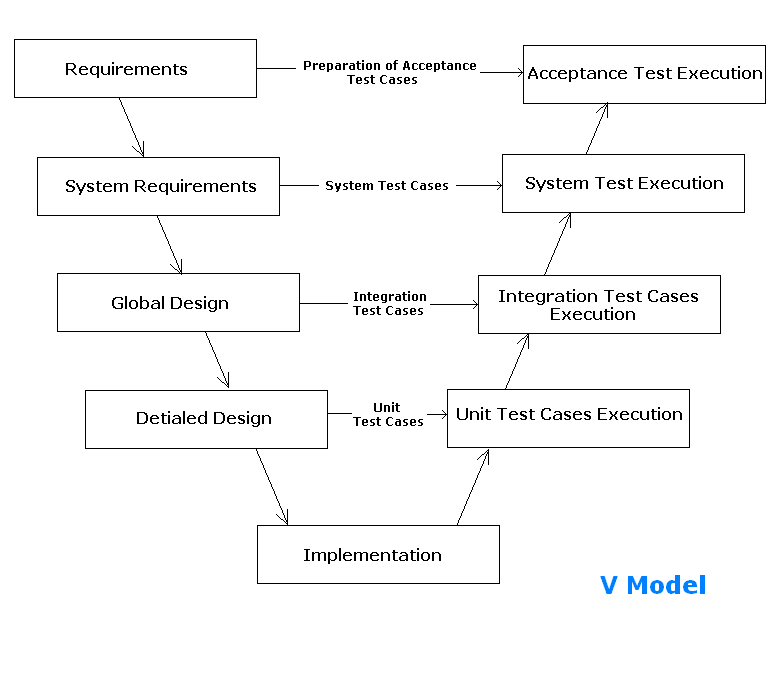
\includegraphics[width=0.9\linewidth]{../img/v-model}
			\caption[Modello a V per collaudo del \mgls{software}]{}
			\label{fig:v-model}
		\end{figure}
		
	Sono definibili 5 tipi diversi di test: test di unità, test di integrazione, test di sistema, test di regressione e test di accettazione o validazione.
	
	\paragraph{Test di unità}
	Consiste nella verifica di ogni singola unità del prodotto \mgls{software} tramite l'utilizzo di \mgls{stub}, \mgls{driver} e \mgls{logger}. Per unità si intende la più piccola quantità di \mgls{software} che è utile verificare singolarmente e che viene prodotta da un singolo programmatore. Ogni test di unità deve essere collegato in modo chiaro alla classe e al metodo testato, grazie all'attività di tracciamento.
	
	\paragraph{Test di integrazione}
	Rispecchia il primo livello della suddivisione modulare del \mgls{software} e si basa sulla correttezza dei test di unità per la diminuzione dei costi di verifica. Verranno pertanto verificati solamente le interazioni tra le varie unità \mgls{software}.
	
	\paragraph{Test di sistema}
	Consiste nella validazione del prodotto giunto a versione definitiva. La correttezza del sistema e dei relativi test è garantita per costruzione dalla struttura gerarchica della suddivisione del \mgls{software}. Il tracciamento dei test di sistema deve rendere chiaro il collegamento tra test di sistema e relativi requisiti del prodotto, alla cui verifica è finalizzato il test.
	\paragraph{Test di regressione}
	Consiste nella trattazione di casi in cui alcune componenti abbiano subito modifiche. Il controllo deve assicurare che non ci siano cambiamenti esterni alle componenti modificate, per garantire l'integrità del prodotto finale modificato.
	
	\paragraph{Test di validazione}
	E' il collaudo del prodotto \mgls{software} che viene eseguito in presenza del \mgls{proponente}. Se tale collaudo viene superato positivamente si può procedere al rilascio ufficiale del prodotto sviluppato. 
	Ogni test di validazione deve mantenere il collegamento, tramite tracciamento, al relativo caso d'uso verificato.
	
	\subsubsection{Strategia di analisi}
	La struttura del sistema di \mgls{collaudo} o analisi deve essere conforme alla struttura del sistema. Tale caratteristica è essenziale per il garantire il funzionamento dell'intero apparato di test. L'esecuzione dei test deve seguire l'ordine cronologico seguente:
	
	\begin{enumerate}
		\item esecuzione e superamento dei test di unità;
		\item esecuzione e superamento dei test di integrazione;
		\item esecuzione e superamento dei test di sistema;
		\item esecuzione e superamento dei test di \mgls{validazione}.
	\end{enumerate}
	
	E' cruciale per l'efficacia dei test che le componenti prodotti non entrino nella fase di test successiva, rispetto a quelle precedentemente esposte, se non soddisfa i test nel punto precedente.
	Inoltre, nel caso di modifiche apportate al software, sarà necessario predisporre opportuni test di regressione.
	\newpage
	
	\section{Misure e metriche}\label{metriche}
	Il processo di verifica, per essere informativo, deve esse quantificabile. Le misure rilevate dal processo di verifica devono quindi essere basate su metriche stabilite a priori. Per ogni metrica utilizzata vi possono essere due tipologie di range:
	
	\begin{itemize}
		\item \textbf{Accettazione:} valori minimi richiesti per superare la verifica di qualità. Scostamenti da tali valori necessitano una verifica approfondita
		\item \textbf{Ottimale:} valori entro cui dovrebbe collocarsi la misurazione. Tale range non è vincolante, ma fortemente consigliato
	\end{itemize}
	
	\subsection{Metriche per i processi}\label{metriche_processi}
	La qualità dei processi viene valutata usando le seguenti metriche.
	
	\subsubsection{Milestone Schedule Variance (MSV)}
	\paragraph{MSV formula generale}
	
	Indica se le scadenze (\mgls{milestone}) stabilite vengono in media rispettate. Lo scopo è quello di valutare l'efficacia della pianificazione preventiva e della gestione dell'organizzazione interna su periodi a lungo termine. Tale metrica si serve del concetto di \mgls{milestone}.
	
	\[MSV [\%] = \frac{SDT - PDT}{PDT}\]
	
	dove: 
	\begin{itemize}
		\item MSV indica \MSV;
		\item SDT (Spent Day Time) indica il numero di giorni lavorativi effettivamente utilizzati;
		\item  PDT indica il numero di giorni lavorativi consecutivi pianificati.
	\end{itemize}
	
 
    PDT indica il numero di giorni lavorativi consecutivi pianificati.
	
	\paragraph{MSV medio per persona}
	\[MSV medio\_persona [\%] = \frac{\sum_{i=0}^n msv_i}{n}\]
		dove:
		\begin{itemize} 
		\item\textbf{ msv\_i} è il \mgls{milestone schedule variance} calcolato per il membro i-esimo del gruppo;
		\item \textbf{n} è il numero di componenti del gruppo.
	\end{itemize}{}
	\paragraph{MSV medio per attività di gruppo}
	\[MSV attivit\acute{a}\_gruppo [\%] = \frac{\sum_{i=0}^n msv_i}{n}\]
			dove: 
			\begin{itemize}
				\item \textbf{msv\_i} è il \mgls{milestone schedule variance} calcolato per una attiivtà completata da più di 1 una persona;
				\item\textbf{ n} è il numero di attività di guppo completate.
			
			\end{itemize}
	
	\paragraph{Range di accettazione}
	\begin{itemize}
		\item \textbf{Primo range di accettazione}: MSV $\leq$ 4.5\%
		\item \textbf{Range Ottimale}: MSV $\leq$ 0\%
	\end{itemize}
	
	L'indice \mgls{milestone schedule variance} valuta l'efficacia della pianificazione a lungo termine e l'affidabilità delle stime relative ai tempi stimati per le \mgls{attivita}  in fase di pianificazione temporale. Tale metrica non valuta la capacità produttiva durante le ore lavorative stimate, ma l'organizzazione del lavoro rispetto al periodo stimato durante la pianificazione.
	
	\subsubsection{Schedule Variance (SV)} \label{schedule_variance}
	Indica se si è in linea, in anticipo o in ritardo rispetto alla pianificazione temporale delle \mgls{attivita}. Il calcolo utilizza le ore lavorative quantificate, ma non tiene conto della loro collocazione nel tempo. Pertanto l'utilizzo di tale metrica risulta utile solamente se le misure effettuate con l'utilizzo della metrica \mgls{milestone schedule variance} hanno risultato positivo.
	
	\[SV [\%] = \frac{ST - PT}{PT}\]
	dove: 
	\begin{itemize}
\item SV indica \mgls{schedule variance} 
\item ST (Spent time) è il valore in ore delle \mgls{attivita}  realizzate alla data corrente;
\item PT (Planned time) è il valore dei ore pianificate per svolgere le stesse le \mgls{attivita}.
\end{itemize}
 Se $SV < 0$ significa che il progetto sta producendo con maggior velocità rispetto a quanto pianificato, viceversa se negativo.
	
	\begin{itemize}
		\item \textbf{Range di Accettazione}: SV $\leq$ 5\%
		\item \textbf{Range Ottimale}: SV $\leq$ 0\%
	\end{itemize}
	
	\subsubsection{Cost Variance (CV)}
	Indica se alla data corrente si è speso di più o di meno rispetto a quanto pianificato.
	
	\[CV [\%] = \frac{EV - AC}{EV}\]
	
	Dove:\begin{itemize}
		\item CV indica \mgls{cost variance};
		\item EV (Earned Value) è il valore in euro delle \mgls{attivita} realizzate alla data corrente;
		\item AC (Actual Cost) equivale ai costi effettivamente sostenuti alla data corrente;
	\end{itemize}  
	
	 Se $CV > 0$ significa che i costi sono entro il budget stabilito, se invece è negativo significa che si sta sforando il budget.
	
	\begin{itemize}
		\item \textbf{Range di Accettazione}: CV $\geq$ -10\%
		\item \textbf{Range Ottimale}: CV $\geq$ 0\%
	\end{itemize}
	
	\subsubsection{Cost of poor quality (CoPQ)}
	Indica l'inefficienza di processi  valutando il costo delle \mgls{attivita} di verifica e l'impatto degli errori non rilevati in fase di verifica  e approvazione sulle \mgls{attivita} successive.
	\paragraph{CoPQ documenti}
	\[CoPQ_{documenti}[\%]= \frac{(sezV*0.25)+sezE}{sezTOT}\]
	\begin{itemize}
		\item sezV indica il numero di sezioni modificate durante la verifica;
		\item sezE indica sezioni con errori modificate dopo l'approvazione.
		\item sezTOT è il numero di sezioni totali.
	\end{itemize}
		\paragraph{CoPQ progettazione}
	\[CoPQ_{progettazione}[\%]=\frac{(classiV*0.25)+classiE}{classiTOT}\]
	\begin{itemize}
		\item classiV indica il numero di classi modificate in verifica;
		\item classiE indica il numero di classi modificate dopo l'approvazione.
		\item classiTOT indica il numero di classi totali.
	\end{itemize}
		\paragraph{CoPQ software}
	\[CoPQ_{software}[\%]= \frac{\mgls{bug}\ trovati}{KLOC\ verificate}\]
	dove KLOC sono migliaia di linee di codice.
		\paragraph{CoPQ generale}
	\[CoPQ_{generale}[\%]= \frac{\sum_{i=1}^3 CoPQ_i}{3}\]
	 viene calcolato come la media dei valori di CoPQ di documenti, progettazione e \mgls{software} definiti  sopra.
	
	\paragraph{Range di accettazione}
	\begin{itemize}
		\item \textbf{Range di Accettazione}: CoPQ $\leq$ 30\%
		\item \textbf{Range Ottimale}:CoPQ $\leq$ 10\%
	\end{itemize}
	
	\subsubsection{Requirement stability index (RSI)}
	Indica quanto variano i requisiti nel tempo.
	
	\[RSI[\%]= 1 - \frac{\#requisiti\ aggiunti+\#requisiti\ tolti+\#requisiti\ modificati}{\#requisiti\ totali\ inizialmente}\]
	
	\begin{itemize}
		\item \textbf{Range di Accettazione}: RSI $\geq$ 80\%
		\item \textbf{Range Ottimale}: RSI $\geq$ 90\%
	\end{itemize}
	
	\subsection{Metriche per i documenti}\label{metriche_doc}
	
	\subsubsection{Gulpease}
	È un indice di leggibilità di un testo tarato sulla lingua italiana.
	
	\[IndiceGulpease=89-\frac{300*(Numero\ di\ frasi)-10*(Numero\ di\ lettere)}{Numero\ di\ parole}\]
	
	Il range di valori è compreso tra 0 e 100, dove il valore 100 indica la leggibilità più alta e 0 la più bassa.
	
	\begin{itemize}
		\item \textbf{Range di Accettazione}: [40-100]
		\item \textbf{Range Ottimale}: [50-100]
	\end{itemize}
	
	\subsection{Metriche per il software}\label{metriche_sw}
	
	\subsubsection{Complessità ciclomatica}
	Misura la complessità del programma contando il numero di cammini linearmente indipendenti attraverso il grafo di controllo di flusso. Valori troppo alti implicano una ridotta manutenibilità del codice, valori troppo bassi potrebbero determinare scarsa efficienza dei metodi.
	
	\begin{itemize}
		\item \textbf{Range di Accettazione}: [1-15]
		\item \textbf{Range Ottimale}: [1-10]
	\end{itemize}
	
	\subsubsection{Numero di parametri per metodo}
	Un numero troppo elevato di parametri per metodo indica una scarsa leggibilità e manutenibilità del codice.
	
	\begin{itemize}
		\item \textbf{Range di Accettazione}: [0-8]
		\item \textbf{Range Ottimale}: [0-4]
	\end{itemize}
	
	\subsubsection{Numero di campi dati per classe}
	Una classe con un numero elevato di campi dati suggerisce che si potrebbe espandere la gerarchia di classi, migliorando l'incapsulamento.
	A causa delle tecnologie utilizzate e delle diverse modalità di progettazione, sono stati definite due diverse tipologie di range di accettazione.
	
	\paragraph{Range di accettazione per classi di tipo "service"}
	Il seguente range di accettazione è specifico per classi di tipo "service" sia lato front-end che lato back-end. Tali classi sono viste come un raggruppamento di funzionalità. La mancanza di uno stato interno alla classe non viene pertanto visto come una forma di cattiva progettazione.
	\begin{itemize}
		\item \textbf{Range di Accettazione}: [0-8]
		\item \textbf{Range Ottimale}: [0-4]
	\end{itemize}
	\paragraph{Range di accettazione generale}
	Il seguente range di accettazione è adatto a tutte le classi che non appartengono alla categoria "servizi". Per questo tipo di classi una mancanza di uno stato interno è interpretabile come frutto di una cattiva progettazione.
	\begin{itemize}
		\item \textbf{Range di Accettazione}: [2-16]
		\item \textbf{Range Ottimale}: [3-8]
	\end{itemize}
	\subsubsection{Numero linee di codice per metodo}
	La complessità dei metodi molte volte è proporzionale alla loro lunghezza, quindi è bene spezzare elaborazioni complesse in più metodi, in modo da facilitarne anche la comprensione.
	
	\begin{itemize}
		\item \textbf{Range di Accettazione}: [1-70]
		\item \textbf{Range Ottimale}: [1-40]
	\end{itemize}
	
	\subsubsection{Numero di livelli di annidamento}
	Rappresenta il massimo numero di livelli di annidamento dei metodi. Un valore elevato di tale indice implica un'alta complessità ed un basso livello di astrazione del codice.
	
	\begin{itemize}
		\item \textbf{Range di Accettazione}: [1-5]
		\item \textbf{Range Ottimale}: [1-3]
	\end{itemize}
	
	\subsubsection{Instabilità}
	La stabilità di una componente indica la possibilità di effettuare modiche ad un componente senza influenzarne altri all'interno dell'applicazione.
	
	\[Instabilita=\frac{A_e}{A_a+A_e}\]
	
	Dove: \begin{itemize}
		\item $A_a$ (Accoppiamento afferente) è il numero di classi esterne ad un \mgls{package} che dipendono da classi interne ad esso;
		\item il $A_e$ (Accoppiamento efferente) è il numero di classi interne al \mgls{package} che dipendono da classi esterne ad esso.
	\end{itemize}  
	
	\begin{itemize}
		\item \textbf{Range di Accettazione}:[0-0.9]
		\item \textbf{Range Ottimale}: [0-0.5]
	\end{itemize}
	
	\subsubsection{Copertura del codice da parte di test}
	Indica la percentuale di istruzioni che sono coperte durante i test. Maggiore è la percentuale di istruzioni coperte dai test eseguiti, maggiore sarà la probabilità che le componenti testate abbiano una ridotta quantità di errori. Il valore di tale indice può essere abbassato da metodi molto semplici che non richiedono alcun \mgls{collaudo}. Esempi di questi metodi sono: get e set.
	
	\begin{itemize}
		\item \textbf{Range di Accettazione}: [50\%-100\%]
		\item \textbf{Range Ottimale}: [75\%-100\%]
	\end{itemize}
	
	\newpage
	\appendix
	
	\section{Test del prodotto software}\label{test}
	\subsection{Notazione}
	\paragraph{Test di Validazione}
	L'identificativo di un test di validazione è attribuito in modo automatico secondo lo schema:
	\[ TV.[ID test ]\]
	dove la sigla TV si riferisce a un test di validazione, [ID test] viene sostituito dall'identificativo numerico, attribuito automaticamente ad ogni test di validazione.
		
	\paragraph{Test di Sistema}
	L'identificativo di un test di sistema è attribuito in modo automatico secondo lo schema:
	\[ TS.[ID req]\]
	dove la sigla TS si riferisce a un test di sistema, [ID req] viene sostituito dall'identificativo numerico del requisito sul sistema.
	 
	\paragraph{Test di Integrazione}
	L'identificativo di un test di integrazione è attribuito in modo automatico secondo lo schema:
	\[ TI.[componete]\]
	dove la sigla TI si riferisce a un test di integrazione, [componente] viene sostituito del macro componente di cui si verifica l'integrazione.
	
	\paragraph{Test di Unità}
L'identificazione dei test sarà invece definita tramite un identificativo proprio del test di unità, in particolare
	\[ TU.[ID Metodo] \] 
	dove ID Metodo rappresenta l'ID del metodo della classe testato.
	 Nel caso il test coinvolga più metodi (sconsigliato), si possono concatenare i vari ID separati dal carattere "-".
	
	\paragraph{Stato dei test}
	Per indicare lo stato dei test si usa la seguente notazione:

	\begin{itemize}
		\item \textbf{NI:} test non implementato
		\item \textbf{I:} test implementato
		\item \textbf{P:} test implementato superato
		\item \textbf{F:} test implementato non superato
	\end{itemize}
		
\subsection{Test di validazione}\label{test_pianificazione}	
	\begin{longtable}{r l p{10cm} l l}
		\midrule
		\multicolumn{2}{c}{\textbf{ID}} & \textbf{Descrizione} & \textbf{Requisito} & \textbf{Stato}\tabularnewline
		\midrule
		\midrule
		& TV1 & Verifica che l'ospite sia in grado di effettuare la registrazione presso il sistema attraverso i seguenti passi:
		
		\begin{enumerate}
			\item accesso alla pagina di registrazione;
			\item immissione dei dati dell'utente;
			\item conferma registrazione.
		\end{enumerate} & R-3F9 & NI\tabularnewline
		\midrule
		& TV2 & Verifica che l'ospite sia in grado di effettuare l'accesso attraverso i passi seguenti:
		
		\begin{enumerate}
			\item accesso alla pagina di login;
			\item inserimento credenziali;
			\item conferma accesso.
		\end{enumerate} & R-3F31 & NI\tabularnewline
		\midrule
		& TV3 & Verifica che uno studente sia in grado di eseguire un questionario attraverso i seguenti passi:
		
		\begin{enumerate}
			\item ricerca questionario;
			\item selezione questionario;
			\item compilazione questionario;
			\item conferma compilazione;
			\item visualizzazione dei risultati.
		\end{enumerate} & R-3F16 & NI\tabularnewline
		\midrule
		& TV4 & Verifica che il docente sia in grado di creare una domanda attraverso i seguenti passi:
		
		\begin{enumerate}
			\item accesso alla pagina di creazione domanda;
			\item scrittura della domanda in QML;
			\item selezione degli argomenti relativi alla domanda;
			\item conferma della creazione della domanda.
		\end{enumerate} & R-3F7.11.1 & NI\tabularnewline
		\midrule
		& TV5 & Verifica che il docente sia in grado di modificare una domanda attraverso i seguenti passi:
		
		\begin{enumerate}
			\item selezione domanda da modificare;
			\item modifica QML domanda;
			\item modifica argomenti domanda;
			\item conferma modifica.
		\end{enumerate} & R-3F7.11.2 & NI\tabularnewline
		\midrule
		& TV6 & Verifica che un docente sia in grado di cancellare una propria domanda non utilizzata da alcun questionario attraverso i seguenti passi:
		
		\begin{enumerate}
			\item selezione domanda da eliminare;
			\item conferma eliminazione domanda.
		\end{enumerate} & R-3F7.11.3 & NI\tabularnewline
		\midrule
		& TV7 & Verifica che un docente sia in grado di creare un questionario attraverso i seguenti passi:
		
		\begin{enumerate}
			\item accesso alla pagina di creazione questionario;
			\item selezione argomenti questionario;
			\item aggiunta domande questionario;
			\item conferma creazione.
		\end{enumerate} & R-3F7.7 & NI\tabularnewline
		\midrule
		& TV8 & Verifica che un docente sia in grado di modificare un proprio questionario attraverso i seguenti passi:
		
		\begin{enumerate}
			\item selezione questionario da modificare;
			\item modifica argomenti del questionario;
			\item modifica lista domande del questionario;
			\item conferma modifica.
		\end{enumerate} & R-3F7.12 & NI\tabularnewline
		\midrule
		& TV9 & Verifica che un docente sia in grado di eliminare un proprio questionario attraverso i seguenti passi:
		
		\begin{enumerate}
			\item selezione questionario;
			\item conferma eliminazione questionario.
		\end{enumerate} & R-3F7.13 & NI\tabularnewline
		\midrule
		& TV10 & Verifica che il docente sia in grado di creare un nuovo argomento attraverso i seguenti passi:
		
		\begin{enumerate}
			\item accesso pagina di aggiunta argomento;
			\item definizione dati argomento;
			\item conferma creazione argomento.
		\end{enumerate} & R-3F22.1 & NI\tabularnewline
		\midrule
		& TV11 & Verifica che un docente sia in grado di modificare un argomento attraverso i seguenti passi:
		
		\begin{enumerate}
			\item selezione argomento da modificare;
			\item modifica dati argomento;
			\item conferma modifica dati argomento.
		\end{enumerate} & R-3F22.3 & NI\tabularnewline
		\midrule
		& TV12 & Verifica che un docente sia in grado di eliminare un argomento attraverso i seguenti passi:
		
		\begin{enumerate}
			\item selezione argomento da eliminare;
			\item conferma eliminazione argomento.
		\end{enumerate} & R-3F22.2 & NI\tabularnewline
		\midrule
		& TV13 & Verifica che un amministratore o proprietario sia in grado di eliminare un utente di ruolo inferiore al proprio attraverso i seguenti passi:
		
		\begin{enumerate}
			\item selezione utente da eliminare;
			\item conferma eliminazione utente.
		\end{enumerate} & R-3F11.2 & NI\tabularnewline
		\midrule
		& TV14 & Verifica che un amministratore o proprietario sia in grado di cambiare il ruolo di un utente di ruolo inferiore al proprio attraverso i seguenti passi:
		
		\begin{enumerate}
			\item selezione utente;
			\item selezione ruolo utente;
			\item conferma modifica ruolo utente.
		\end{enumerate} & R-3F11.1 & NI\tabularnewline
		\midrule
		& TV15 & Verifica che un utente sia in grado di aggiornare i propri dati personali attraverso i seguenti passi:
		
		\begin{enumerate}
			\item accesso profilo utente;
			\item accesso pagina di modifica profilo;
			\item modifica dati personali;
			\item conferma modifica.
		\end{enumerate} & R-3F13.3 & NI\tabularnewline
		\midrule
		& TV16 & Verifica che un utente sia in grado di modificare la propria password attraverso i seguenti passi:
		
		\begin{enumerate}
			\item accesso profilo;
			\item selezione modifica password;
			\item inserimento vecchia password;
			\item inserimento nuova password;
			\item inserimento nuova password una seconda volta;
			\item conferma modifica password.
		\end{enumerate} & R-3F13.2 & NI\tabularnewline
		\midrule
		& TV17 & Verifica che un utente sia in grado di disconnettersi dal sistema attraverso i seguenti passi:
		
		\begin{enumerate}
			\item accesso profilo;
			\item conferma disconnessione.
		\end{enumerate} & R-3F17 & NI\tabularnewline
		\midrule
		& TV18 & Verifica che un amministratore o proprietario sia in grado di visualizzare la lista degli utenti, eventualmente specificando parametri per il filtraggio del risultati, attraverso i seguenti passi:
		
		\begin{enumerate}
			\item accesso lista utenti;
			\item specifica parametri di filtraggio dei risultati;
			\item visualizzazione elenco.
		\end{enumerate} & R-3F32 & NI\tabularnewline
		\midrule
		& TV19 & Verifica che un docente sia in grado di visualizzare la lista degli argomenti, eventualmente specificando parametri per il filtraggio del risultati, attraverso i seguenti passi:
		
		\begin{enumerate}
			\item accesso lista argomenti;
			\item specifica parametri di filtraggio dei risultati;
			\item visualizzazione elenco.
		\end{enumerate} & R-3F22.4 & NI\tabularnewline
		\midrule
		& TV20 & Verifica che un docente sia in grado di visualizzare la lista delle domande, eventualmente specificando parametri per il filtraggio del risultati, attraverso i seguenti passi:
		
		\begin{enumerate}
			\item accesso lista domande;
			\item specifica parametri di filtraggio dei risultati;
			\item visualizzazione elenco.
		\end{enumerate} & R-3F19 & NI\tabularnewline
		\midrule
		& TV21 & Verifica che un utente sia in grado di visualizzare la lista dei questionari, eventualmente specificando parametri per il filtraggio del risultati, attraverso i seguenti passi:
		
		\begin{enumerate}
			\item accesso lista questionari;
			\item specifica parametri di filtraggio dei risultati;
			\item visualizzazione elenco.
		\end{enumerate} & R-3F14 & NI\tabularnewline
		\midrule
		& TV22 & Verifica che il docente sia in grado di visualizzare una domanda attraverso i passi seguenti: \begin{enumerate} \item selezione della domanda; \item visualizzazione dati domanda. \end{enumerate} & R-3F29 & NI\tabularnewline
		\midrule
		& TV23 & Verifica che il docente sia in grado di visualizzare un questionario attraverso i passi seguenti: \begin{enumerate} \item selezione del questionario; \item visualizzazione dati e elenco domande questionario. \end{enumerate} & R-3F30 & NI\tabularnewline
		\midrule
		\caption{Tabella test validazione / requisiti} \tabularnewline
	\end{longtable}
	\subsection{Test di sistema}\label{test_sistema}

\begin{longtable}{l p{9cm} l l}
\midrule
\textbf{ID} & \textbf{Descrizione} & \textbf{Stato} & \textbf{Requisito} \tabularnewline
\midrule
\midrule
		TS7.5 & I sotto-requisiti obbligatori sono verificati e viene verificato che il QML riesca a descrivere in maniera efficace tutte le caratteristiche previste per un questionario e le relative domande & P& \hypertarget{R-3F7.5}{R-3F7.5}\tabularnewline
		\midrule
		TS7.5.1 & I sotto-requisiti obbligatori sono verificati e viene verificato che il QML permetta di definire il testo di una domanda e delle relative risposte attraverso una sintassi univoca & P& \hypertarget{R-3F7.5.1}{R-3F7.5.1}\tabularnewline
		\midrule
		TS7.5.1.2 & Viene verificato che il QML permetta l'inserimento di immagini & NI & \hypertarget{R-3F7.5.1.2}{R-3F7.5.1.2}\tabularnewline
		\midrule
		TS7.5.1.6 & Viene verificato che il QML permetta di definire vari tipi di domanda & NI & \hypertarget{R-3F7.5.1.6}{R-3F7.5.1.6}\tabularnewline
		\midrule
		TS7.5.3 & Viene verificato che le domande in QML possano essere scritte e modificate da un docente & P& \hypertarget{R-3F7.5.3}{R-3F7.5.3}\tabularnewline
		\midrule
		TS7.5.5 & Viene verificato che Il QML possa gestire risposte vero/falso, risposte a scelta multipla, possa contenere testi e immagini	 & NI & \hypertarget{R-3F7.5.5}{R-3F7.5.5}\tabularnewline
		\midrule
		TS7.7 & Viene verificato che un docente possa costruire un nuovo questionario utilizzando le domande presenti nel sistema e che non sia possibile creare un questionario che non contenga domande o argomenti
		& P& \hypertarget{R-3F7.7}{R-3F7.7}\tabularnewline
		\midrule
		TS7.11 & Viene verificato che sia possibile per un docente eseguire le operazioni di inserimento, modifica e rimozione di una domanda e che tutti i casi non corretti vengano segnalati & P& \hypertarget{R-3F7.11}{R-3F7.11}\tabularnewline
		\midrule
		TS7.11.1.2.1 & Viene verificato che il sistema sia in grado di verificare l'inserimento di QML valido e, in caso contrario, segnalare un errore & NI & \hypertarget{R-3F7.11.1.2.1}{R-3F7.11.1.2.1}\tabularnewline
		\midrule
		TS7.11.1.2.2 & Viene verificato che il docente possa inserire domande di tipo vero/falso	 & P& \hypertarget{R-3F7.11.1.2.2}{R-3F7.11.1.2.2}\tabularnewline
		\midrule
		TS7.11.1.2.4 & Viene verificato che il docente possa inserire domande di tipo scelta multipla & NI & \hypertarget{R-1F7.11.1.2.4}{R-1F7.11.1.2.4}\tabularnewline
		\midrule
		TS7.12 & Viene verificato che sia possibile per un docente modificare un questionario che ha precedentemente creato & NI & \hypertarget{R-3F7.12}{R-3F7.12}\tabularnewline
		\midrule
		TS7.13 & Viene verificato che sia possibile per un docente eliminare un questionario che ha precedentemente creato & NI & \hypertarget{R-3F7.13}{R-3F7.13}\tabularnewline
		\midrule
		TS8 & Viene verificato che il sistema possa gestire l'accesso e la registrazione di ogni tipo di utente previsto & P& \hypertarget{R-3F8}{R-3F8}\tabularnewline
		\midrule
		TS9 & Viene verificato che sia possibile per ogni tipo di utente registrarsi presso il sistema & NI & \hypertarget{R-3F9}{R-3F9}\tabularnewline
		\midrule
		TS9.1 & Viene verificato che il sistema consenta le funzionalità utente solo se possiede un proprietario & NI & \hypertarget{R-3F9.1}{R-3F9.1}\tabularnewline
		\midrule
		TS9.2 & I sotto-requisiti sono verificati. Viene verificato che sia possibile per un utente registrarsi presso il sistema con una password e le proprie informazioni personali & P& \hypertarget{R-3F9.2}{R-3F9.2}\tabularnewline
		\midrule
		TS9.2.1 & Viene verificato che il sistema segnali un errore se non vengono inseriti tutti i campi necessari alla registrazione di un utente & NI & \hypertarget{R-3F9.2.1}{R-3F9.2.1}\tabularnewline
		\midrule
		TS11 & Viene verificato che il sistema gestisca correttamente tutte le funzionalità di un amministratore & P& \hypertarget{R-3F11}{R-3F11}\tabularnewline
		\midrule
		TS13 & Viene verificato che il sistema consenta ad un utente di modificare le proprie informazioni personali presenti nel sistema & P& \hypertarget{R-3F13}{R-3F13}\tabularnewline
		\midrule
		TS14 & Viene verificato che, per ogni tipo di utente, il sistema gestisca correttamente la ricerca di un questionario da parte di un utente & NI & \hypertarget{R-3F14}{R-3F14}\tabularnewline
		\midrule
		TS16 & Viene verificato che un utente sia in grado di rispondere alle domande di un questionario & P& \hypertarget{R-3F16}{R-3F16}\tabularnewline
		\midrule
		TS17 & Viene verificato che per un qualsiasi tipo di utente autenticato presso il sistema sia possibile effettuare correttamente il log-out  & P& \hypertarget{R-3F17}{R-3F17}\tabularnewline
		\midrule
		TS18 & Viene verificato che il sistema consenta e gestisca correttamente tutte le azioni previste per il proprietario & NI & \hypertarget{R-3F18}{R-3F18}\tabularnewline
		\midrule
		TS19 & Viene verificato che per un docente sia possibile effettuare correttamente la ricerca di una domanda presente nel sistema & P& \hypertarget{R-3F19}{R-3F19}\tabularnewline
		\midrule
		TS22 & Viene verificato che sia possibile per un docente, amministratore e proprietario la gestione degli argomenti presenti nel sistema & NI & \hypertarget{R-3F22}{R-3F22}\tabularnewline
		\midrule
		TS29 & Viene verificato che il sistema consenta ad un docente di visualizzare una domanda & P& \hypertarget{R-3F29}{R-3F29}\tabularnewline
		\midrule
		TS30 & Viene verificato che il sistema consenta ad un docente di visualizzare un questionario & NI & \hypertarget{R-3F30}{R-3F30}\tabularnewline 	\midrule 
		\caption{Tabella di tracciamento test di sistema / requisiti} \tabularnewline
	\end{longtable}
	
	\subsubsection{Tracciamento TS-Requisito}
	\begin{longtable}{r l l}
		\midrule
		\multicolumn{2}{c}{\textbf{Requisito}} & \textbf{Test} \tabularnewline
		\midrule
		\midrule
		& R-3V1 & Il resposabile certifica questo requisito\tabularnewline
		\midrule
		& R-3V2 & Il resposabile certifica questo requisito\tabularnewline
		\midrule
		& R-3V3 & Validatore w3c\tabularnewline
		\midrule
		\begin{tikzpicture}
		\draw [->, thick] (0.2,0.2) -- (0.2,0.1) -- (1,0.1);
		\end{tikzpicture} & R-3V3.1 & test prodotto su browser specificato\tabularnewline
		\midrule
		\begin{tikzpicture}
		\draw [->, thick] (0.2,0.2) -- (0.2,0.1) -- (1,0.1);
		\end{tikzpicture} & R-3V3.2 & Validatore w3c\tabularnewline
		\midrule
		\begin{tikzpicture}
		\draw [->, thick] (0.2,0.2) -- (0.2,0.1) -- (1,0.1);
		\end{tikzpicture} & R-3V3.3 & test prodotto su browser specificato\tabularnewline
		\midrule
		\begin{tikzpicture}
		\draw [->, thick] (0.2,0.2) -- (0.2,0.1) -- (1,0.1);
		\end{tikzpicture} & R-3V3.4 & I moduli superano test unità, verifica use cases relativi\tabularnewline
		\midrule
		& R-3V4 & Il resposabile certifica questo requisito\tabularnewline
		\midrule
		& R-3V5 & Il resposabile certifica questo requisito\tabularnewline
		\midrule
		& R-3V6 & Il sistema utilizza tecnologie supportate su tali dispositivi\tabularnewline
		\midrule
		\begin{tikzpicture}
		\draw [->, thick] (0.2,0.2) -- (0.2,0.1) -- (1,0.1);
		\end{tikzpicture} & R-3V6.1 & Il sistema utilizza tecnologie supportate su tali dispositivi\tabularnewline
		\midrule
		\begin{tikzpicture}
		\draw [->, thick] (0.2,0.2) -- (0.2,0.1) -- (1,0.1);
		\end{tikzpicture} & R-3V6.2 & Il sistema utilizza tecnologie supportate su tali dispositivi\tabularnewline
		\midrule
		& R-3F7 & I moduli superano test unità, verifica use cases relativi\tabularnewline
		\midrule
		\begin{tikzpicture}
		\draw [->, thick] (0.2,0.2) -- (0.2,0.1) -- (1,0.1);
		\end{tikzpicture} & R-3F7.1 & I moduli superano test unità, verifica use cases relativi\tabularnewline
		\midrule
		\begin{tikzpicture}
		\draw [->, thick] (0.2,0.2) -- (0.2,0.1) -- (1,0.1);
		\end{tikzpicture} & R-3F7.2 & I moduli superano test unità, verifica use cases relativi\tabularnewline
		\midrule
		\begin{tikzpicture}
		\draw [->, thick] (0.2,0.2) -- (0.2,0.1) -- (1,0.1);
		\end{tikzpicture} & R-3F7.3 & I moduli superano test unità, verifica use cases relativi\tabularnewline
		\midrule
		\begin{tikzpicture}
		\draw [->, thick] (0.2,0.2) -- (0.2,0.1) -- (1,0.1);
		\end{tikzpicture} & R-3F7.4 & I moduli superano test unità, verifica use cases relativi\tabularnewline
		\midrule
		\begin{tikzpicture}
		\draw [->, thick] (0.2,0.2) -- (0.2,0.1) -- (1,0.1);
		\end{tikzpicture} & R-3F7.5 & TS7.5\tabularnewline
		\midrule
		\begin{tikzpicture}
		\draw [->, thick] (0.4,0.2) -- (0.4,0.1) -- (1,0.1);
		\end{tikzpicture} & R-3F7.5.1 & TS7.5.1\tabularnewline
		\midrule
		\begin{tikzpicture}
		\draw [->, thick] (0.6,0.2) -- (0.6,0.1) -- (1,0.1);
		\end{tikzpicture} & R-2F7.5.1.1 & I moduli superano test unità, verifica use cases relativi\tabularnewline
		\midrule
		\begin{tikzpicture}
		\draw [->, thick] (0.6,0.2) -- (0.6,0.1) -- (1,0.1);
		\end{tikzpicture} & R-3F7.5.1.2 & TS7.5.1.2\tabularnewline
		\midrule
		\begin{tikzpicture}
		\draw [->, thick] (0.6,0.2) -- (0.6,0.1) -- (1,0.1);
		\end{tikzpicture} & R-2F7.5.1.3 & I moduli superano test unità, verifica use cases relativi\tabularnewline
		\midrule
		\begin{tikzpicture}
		\draw [->, thick] (0.6,0.2) -- (0.6,0.1) -- (1,0.1);
		\end{tikzpicture} & R-2F7.5.1.4 & I moduli superano test unità, verifica use cases relativi\tabularnewline
		\midrule
		\begin{tikzpicture}
		\draw [->, thick] (0.6,0.2) -- (0.6,0.1) -- (1,0.1);
		\end{tikzpicture} & R-2F7.5.1.5 & I moduli superano test unità, verifica use cases relativi\tabularnewline
		\midrule
		\begin{tikzpicture}
		\draw [->, thick] (0.6,0.2) -- (0.6,0.1) -- (1,0.1);
		\end{tikzpicture} & R-3F7.5.1.6 & TS7.5.1.6\tabularnewline
		\midrule
		\begin{tikzpicture}
		\draw [->, thick] (0.6,0.2) -- (0.6,0.1) -- (1,0.1);
		\end{tikzpicture} & R-2F7.5.1.7 & I moduli superano test unità, verifica use cases relativi\tabularnewline
		\midrule
		\begin{tikzpicture}
		\draw [->, thick] (0.6,0.2) -- (0.6,0.1) -- (1,0.1);
		\end{tikzpicture} & R-2F7.5.1.8 & I moduli superano test unità, verifica use cases relativi\tabularnewline
		\midrule
		\begin{tikzpicture}
		\draw [->, thick] (0.4,0.2) -- (0.4,0.1) -- (1,0.1);
		\end{tikzpicture} & R-2F7.5.2 & I moduli superano test unità, verifica use cases relativi\tabularnewline
		\midrule
		\begin{tikzpicture}
		\draw [->, thick] (0.4,0.2) -- (0.4,0.1) -- (1,0.1);
		\end{tikzpicture} & R-3F7.5.3 & TS7.5.3\tabularnewline
		\midrule
		\begin{tikzpicture}
		\draw [->, thick] (0.4,0.2) -- (0.4,0.1) -- (1,0.1);
		\end{tikzpicture} & R-2F7.5.4 & I moduli superano test unità, verifica use cases relativi\tabularnewline
		\midrule
		\begin{tikzpicture}
		\draw [->, thick] (0.4,0.2) -- (0.4,0.1) -- (1,0.1);
		\end{tikzpicture} & R-3F7.5.5 & TS7.5.5\tabularnewline
		\midrule
		\begin{tikzpicture}
		\draw [->, thick] (0.2,0.2) -- (0.2,0.1) -- (1,0.1);
		\end{tikzpicture} & R-2F7.6 & I moduli superano test unità, verifica use cases relativi\tabularnewline
		\midrule
		\begin{tikzpicture}
		\draw [->, thick] (0.2,0.2) -- (0.2,0.1) -- (1,0.1);
		\end{tikzpicture} & R-3F7.7 & TS7.7\tabularnewline
		\midrule
		\begin{tikzpicture}
		\draw [->, thick] (0.4,0.2) -- (0.4,0.1) -- (1,0.1);
		\end{tikzpicture} & R-3F7.7.1 & I moduli superano test unità, verifica use cases relativi\tabularnewline
		\midrule
		\begin{tikzpicture}
		\draw [->, thick] (0.2,0.2) -- (0.2,0.1) -- (1,0.1);
		\end{tikzpicture} & R-2F7.8 & I moduli superano test unità, verifica use cases relativi\tabularnewline
		\midrule
		\begin{tikzpicture}
		\draw [->, thick] (0.2,0.2) -- (0.2,0.1) -- (1,0.1);
		\end{tikzpicture} & R-2F7.9 & I moduli superano test unità, verifica use cases relativi\tabularnewline
		\midrule
		\begin{tikzpicture}
		\draw [->, thick] (0.2,0.2) -- (0.2,0.1) -- (1,0.1);
		\end{tikzpicture} & R-2F7.10 & I moduli superano test unità, verifica use cases relativi\tabularnewline
		\midrule
		\begin{tikzpicture}
		\draw [->, thick] (0.4,0.2) -- (0.4,0.1) -- (1,0.1);
		\end{tikzpicture} & R-2F7.10.1 & I moduli superano test unità, verifica use cases relativi\tabularnewline
		\midrule
		\begin{tikzpicture}
		\draw [->, thick] (0.4,0.2) -- (0.4,0.1) -- (1,0.1);
		\end{tikzpicture} & R-2F7.10.2 & I moduli superano test unità, verifica use cases relativi\tabularnewline
		\midrule
		\begin{tikzpicture}
		\draw [->, thick] (0.4,0.2) -- (0.4,0.1) -- (1,0.1);
		\end{tikzpicture} & R-2F7.10.3 & I moduli superano test unità, verifica use cases relativi\tabularnewline
		\midrule
		\begin{tikzpicture}
		\draw [->, thick] (0.2,0.2) -- (0.2,0.1) -- (1,0.1);
		\end{tikzpicture} & R-3F7.11 & TS7.11\tabularnewline
		\midrule
		\begin{tikzpicture}
		\draw [->, thick] (0.4,0.2) -- (0.4,0.1) -- (1,0.1);
		\end{tikzpicture} & R-3F7.11.1 & I moduli superano test unità, verifica use cases relativi\tabularnewline
		\midrule
		\begin{tikzpicture}
		\draw [->, thick] (0.6,0.2) -- (0.6,0.1) -- (1,0.1);
		\end{tikzpicture} & R-3F7.11.1.1 & I moduli superano test unità, verifica use cases relativi\tabularnewline
		\midrule
		\begin{tikzpicture}
		\draw [->, thick] (0.8,0.2) -- (0.8,0.1) -- (1,0.1);
		\end{tikzpicture} & R-3F7.11.1.1.1 & I moduli superano test unità, verifica use cases relativi\tabularnewline
		\midrule
		\begin{tikzpicture}
		\draw [->, thick] (0.6,0.2) -- (0.6,0.1) -- (1,0.1);
		\end{tikzpicture} & R-3F7.11.1.2 & I moduli superano test unità, verifica use cases relativi\tabularnewline
		\midrule
		\begin{tikzpicture}
		\draw [->, thick] (0.8,0.2) -- (0.8,0.1) -- (1,0.1);
		\end{tikzpicture} & R-3F7.11.1.2.1 & TS7.11.1.2.1\tabularnewline
		\midrule
		\begin{tikzpicture}
		\draw [->, thick] (0.8,0.2) -- (0.8,0.1) -- (1,0.1);
		\end{tikzpicture} & R-3F7.11.1.2.2 & TS7.11.1.2.2\tabularnewline
		\midrule
		\begin{tikzpicture}
		\draw [->, thick] (0.8,0.2) -- (0.8,0.1) -- (1,0.1);
		\end{tikzpicture} & R-3F7.11.1.2.3 & I moduli superano test unità, verifica use cases relativi\tabularnewline
		\midrule
		\begin{tikzpicture}
		\draw [->, thick] (0.8,0.2) -- (0.8,0.1) -- (1,0.1);
		\end{tikzpicture} & R-1F7.11.1.2.4 & TS7.11.1.2.4\tabularnewline
		\midrule
		\begin{tikzpicture}
		\draw [->, thick] (0.8,0.2) -- (0.8,0.1) -- (1,0.1);
		\end{tikzpicture} & R-1F7.11.1.2.5 & I moduli superano test unità, verifica use cases relativi\tabularnewline
		\midrule
		\begin{tikzpicture}
		\draw [->, thick] (0.8,0.2) -- (0.8,0.1) -- (1,0.1);
		\end{tikzpicture} & R-1F7.11.1.2.6 & I moduli superano test unità, verifica use cases relativi\tabularnewline
		\midrule
		\begin{tikzpicture}
		\draw [->, thick] (0.8,0.2) -- (0.8,0.1) -- (1,0.1);
		\end{tikzpicture} & R-2F7.11.1.2.7 & I moduli superano test unità, verifica use cases relativi\tabularnewline
		\midrule
		\begin{tikzpicture}
		\draw [->, thick] (0.4,0.2) -- (0.4,0.1) -- (1,0.1);
		\end{tikzpicture} & R-3F7.11.2 & I moduli superano test unità, verifica use cases relativi\tabularnewline
		\midrule
		\begin{tikzpicture}
		\draw [->, thick] (0.4,0.2) -- (0.4,0.1) -- (1,0.1);
		\end{tikzpicture} & R-3F7.11.3 & I moduli superano test unità, verifica use cases relativi\tabularnewline
		\midrule
		\begin{tikzpicture}
		\draw [->, thick] (0.2,0.2) -- (0.2,0.1) -- (1,0.1);
		\end{tikzpicture} & R-3F7.12 & TS7.12\tabularnewline
		\midrule
		\begin{tikzpicture}
		\draw [->, thick] (0.4,0.2) -- (0.4,0.1) -- (1,0.1);
		\end{tikzpicture} & R-3F7.12.1 & I moduli superano test unità, verifica use cases relativi\tabularnewline
		\midrule
		\begin{tikzpicture}
		\draw [->, thick] (0.4,0.2) -- (0.4,0.1) -- (1,0.1);
		\end{tikzpicture} & R-3F7.12.2 & I moduli superano test unità, verifica use cases relativi\tabularnewline
		\midrule
		\begin{tikzpicture}
		\draw [->, thick] (0.4,0.2) -- (0.4,0.1) -- (1,0.1);
		\end{tikzpicture} & R-3F7.12.3 & I moduli superano test unità, verifica use cases relativi\tabularnewline
		\midrule
		\begin{tikzpicture}
		\draw [->, thick] (0.4,0.2) -- (0.4,0.1) -- (1,0.1);
		\end{tikzpicture} & R-3F7.12.4 & I moduli superano test unità, verifica use cases relativi\tabularnewline
		\midrule
		\begin{tikzpicture}
		\draw [->, thick] (0.2,0.2) -- (0.2,0.1) -- (1,0.1);
		\end{tikzpicture} & R-3F7.13 & TS7.13\tabularnewline
		\midrule
		& R-3F8 & TS8\tabularnewline
		\midrule
		& R-3F9 & TS9\tabularnewline
		\midrule
		\begin{tikzpicture}
		\draw [->, thick] (0.2,0.2) -- (0.2,0.1) -- (1,0.1);
		\end{tikzpicture} & R-3F9.1 & TS9.1\tabularnewline
		\midrule
		\begin{tikzpicture}
		\draw [->, thick] (0.2,0.2) -- (0.2,0.1) -- (1,0.1);
		\end{tikzpicture} & R-3F9.2 & TS9.2\tabularnewline
		\midrule
		\begin{tikzpicture}
		\draw [->, thick] (0.4,0.2) -- (0.4,0.1) -- (1,0.1);
		\end{tikzpicture} & R-3F9.2.1 & TS9.2.1\tabularnewline
		\midrule
		\begin{tikzpicture}
		\draw [->, thick] (0.4,0.2) -- (0.4,0.1) -- (1,0.1);
		\end{tikzpicture} & R-3F9.2.2 & I moduli superano test unità, verifica use cases relativi\tabularnewline
		\midrule
		\begin{tikzpicture}
		\draw [->, thick] (0.2,0.2) -- (0.2,0.1) -- (1,0.1);
		\end{tikzpicture} & R-3F9.3 & I moduli superano test unità, verifica use cases relativi\tabularnewline
		\midrule
		\begin{tikzpicture}
		\draw [->, thick] (0.2,0.2) -- (0.2,0.1) -- (1,0.1);
		\end{tikzpicture} & R-3F9.4 & I moduli superano test unità, verifica use cases relativi\tabularnewline
		\midrule
		\begin{tikzpicture}
		\draw [->, thick] (0.2,0.2) -- (0.2,0.1) -- (1,0.1);
		\end{tikzpicture} & R-3F9.5 & I moduli superano test unità, verifica use cases relativi\tabularnewline
		\midrule
		& R-3V10 & I moduli superano test unità, verifica use cases relativi\tabularnewline
		\midrule
		& R-3F11 & TS11\tabularnewline
		\midrule
		\begin{tikzpicture}
		\draw [->, thick] (0.2,0.2) -- (0.2,0.1) -- (1,0.1);
		\end{tikzpicture} & R-3F11.1 & I moduli superano test unità, verifica use cases relativi\tabularnewline
		\midrule
		\begin{tikzpicture}
		\draw [->, thick] (0.2,0.2) -- (0.2,0.1) -- (1,0.1);
		\end{tikzpicture} & R-3F11.2 & I moduli superano test unità, verifica use cases relativi\tabularnewline
		\midrule
		& R-2F12 & I moduli superano test unità, verifica use cases relativi\tabularnewline
		\midrule
		\begin{tikzpicture}
		\draw [->, thick] (0.2,0.2) -- (0.2,0.1) -- (1,0.1);
		\end{tikzpicture} & R-2F12.1 & I moduli superano test unità, verifica use cases relativi\tabularnewline
		\midrule
		\begin{tikzpicture}
		\draw [->, thick] (0.4,0.2) -- (0.4,0.1) -- (1,0.1);
		\end{tikzpicture} & R-2F12.1.1 & I moduli superano test unità, verifica use cases relativi\tabularnewline
		\midrule
		\begin{tikzpicture}
		\draw [->, thick] (0.6,0.2) -- (0.6,0.1) -- (1,0.1);
		\end{tikzpicture} & R-2F12.1.1.1 & I moduli superano test unità, verifica use cases relativi\tabularnewline
		\midrule
		\begin{tikzpicture}
		\draw [->, thick] (0.4,0.2) -- (0.4,0.1) -- (1,0.1);
		\end{tikzpicture} & R-2F12.1.2 & I moduli superano test unità, verifica use cases relativi\tabularnewline
		\midrule
		\begin{tikzpicture}
		\draw [->, thick] (0.4,0.2) -- (0.4,0.1) -- (1,0.1);
		\end{tikzpicture} & R-2F12.1.3 & I moduli superano test unità, verifica use cases relativi\tabularnewline
		\midrule
		\begin{tikzpicture}
		\draw [->, thick] (0.2,0.2) -- (0.2,0.1) -- (1,0.1);
		\end{tikzpicture} & R-2F12.2 & I moduli superano test unità, verifica use cases relativi\tabularnewline
		\midrule
		\begin{tikzpicture}
		\draw [->, thick] (0.2,0.2) -- (0.2,0.1) -- (1,0.1);
		\end{tikzpicture} & R-2F12.3 & I moduli superano test unità, verifica use cases relativi\tabularnewline
		\midrule
		\begin{tikzpicture}
		\draw [->, thick] (0.4,0.2) -- (0.4,0.1) -- (1,0.1);
		\end{tikzpicture} & R-2F12.3.1 & I moduli superano test unità, verifica use cases relativi\tabularnewline
		\midrule
		\begin{tikzpicture}
		\draw [->, thick] (0.4,0.2) -- (0.4,0.1) -- (1,0.1);
		\end{tikzpicture} & R-2F12.3.2 & I moduli superano test unità, verifica use cases relativi\tabularnewline
		\midrule
		\begin{tikzpicture}
		\draw [->, thick] (0.4,0.2) -- (0.4,0.1) -- (1,0.1);
		\end{tikzpicture} & R-2F12.3.3 & I moduli superano test unità, verifica use cases relativi\tabularnewline
		\midrule
		& R-3F13 & TS13\tabularnewline
		\midrule
		\begin{tikzpicture}
		\draw [->, thick] (0.2,0.2) -- (0.2,0.1) -- (1,0.1);
		\end{tikzpicture} & R-3F13.1 & I moduli superano test unità, verifica use cases relativi\tabularnewline
		\midrule
		\begin{tikzpicture}
		\draw [->, thick] (0.4,0.2) -- (0.4,0.1) -- (1,0.1);
		\end{tikzpicture} & R-3F13.1.1 & I moduli superano test unità, verifica use cases relativi\tabularnewline
		\midrule
		\begin{tikzpicture}
		\draw [->, thick] (0.4,0.2) -- (0.4,0.1) -- (1,0.1);
		\end{tikzpicture} & R-3F13.1.2 & I moduli superano test unità, verifica use cases relativi\tabularnewline
		\midrule
		\begin{tikzpicture}
		\draw [->, thick] (0.2,0.2) -- (0.2,0.1) -- (1,0.1);
		\end{tikzpicture} & R-3F13.2 & I moduli superano test unità, verifica use cases relativi\tabularnewline
		\midrule
		\begin{tikzpicture}
		\draw [->, thick] (0.4,0.2) -- (0.4,0.1) -- (1,0.1);
		\end{tikzpicture} & R-3F13.2.1 & I moduli superano test unità, verifica use cases relativi\tabularnewline
		\midrule
		\begin{tikzpicture}
		\draw [->, thick] (0.6,0.2) -- (0.6,0.1) -- (1,0.1);
		\end{tikzpicture} & R-3F13.2.1.1 & I moduli superano test unità, verifica use cases relativi\tabularnewline
		\midrule
		\begin{tikzpicture}
		\draw [->, thick] (0.4,0.2) -- (0.4,0.1) -- (1,0.1);
		\end{tikzpicture} & R-3F13.2.2 & I moduli superano test unità, verifica use cases relativi\tabularnewline
		\midrule
		\begin{tikzpicture}
		\draw [->, thick] (0.6,0.2) -- (0.6,0.1) -- (1,0.1);
		\end{tikzpicture} & R-3F13.2.2.1 & I moduli superano test unità, verifica use cases relativi\tabularnewline
		\midrule
		\begin{tikzpicture}
		\draw [->, thick] (0.2,0.2) -- (0.2,0.1) -- (1,0.1);
		\end{tikzpicture} & R-3F13.3 & I moduli superano test unità, verifica use cases relativi\tabularnewline
		\midrule
		\begin{tikzpicture}
		\draw [->, thick] (0.4,0.2) -- (0.4,0.1) -- (1,0.1);
		\end{tikzpicture} & R-3F13.3.1 & I moduli superano test unità, verifica use cases relativi\tabularnewline
		\midrule
		\begin{tikzpicture}
		\draw [->, thick] (0.4,0.2) -- (0.4,0.1) -- (1,0.1);
		\end{tikzpicture} & R-3F13.3.2 & I moduli superano test unità, verifica use cases relativi\tabularnewline
		\midrule
		\begin{tikzpicture}
		\draw [->, thick] (0.4,0.2) -- (0.4,0.1) -- (1,0.1);
		\end{tikzpicture} & R-3F13.3.3 & I moduli superano test unità, verifica use cases relativi\tabularnewline
		\midrule
		\begin{tikzpicture}
		\draw [->, thick] (0.4,0.2) -- (0.4,0.1) -- (1,0.1);
		\end{tikzpicture} & R-3F13.3.4 & I moduli superano test unità, verifica use cases relativi\tabularnewline
		\midrule
		& R-3F14 & TS14\tabularnewline
		\midrule
		\begin{tikzpicture}
		\draw [->, thick] (0.2,0.2) -- (0.2,0.1) -- (1,0.1);
		\end{tikzpicture} & R-3F14.1 & I moduli superano test unità, verifica use cases relativi\tabularnewline
		\midrule
		\begin{tikzpicture}
		\draw [->, thick] (0.2,0.2) -- (0.2,0.1) -- (1,0.1);
		\end{tikzpicture} & R-2F14.2 & I moduli superano test unità, verifica use cases relativi\tabularnewline
		\midrule
		\begin{tikzpicture}
		\draw [->, thick] (0.2,0.2) -- (0.2,0.1) -- (1,0.1);
		\end{tikzpicture} & R-3F14.3 & I moduli superano test unità, verifica use cases relativi\tabularnewline
		\midrule
		\begin{tikzpicture}
		\draw [->, thick] (0.2,0.2) -- (0.2,0.1) -- (1,0.1);
		\end{tikzpicture} & R-3F14.4 & I moduli superano test unità, verifica use cases relativi\tabularnewline
		\midrule
		\begin{tikzpicture}
		\draw [->, thick] (0.2,0.2) -- (0.2,0.1) -- (1,0.1);
		\end{tikzpicture} & R-2F14.5 & I moduli superano test unità, verifica use cases relativi\tabularnewline
		\midrule
		& R-2F15 & I moduli superano test unità, verifica use cases relativi\tabularnewline
		\midrule
		\begin{tikzpicture}
		\draw [->, thick] (0.2,0.2) -- (0.2,0.1) -- (1,0.1);
		\end{tikzpicture} & R-2F15.1 & I moduli superano test unità, verifica use cases relativi\tabularnewline
		\midrule
		\begin{tikzpicture}
		\draw [->, thick] (0.4,0.2) -- (0.4,0.1) -- (1,0.1);
		\end{tikzpicture} & R-2F15.1.1 & I moduli superano test unità, verifica use cases relativi\tabularnewline
		\midrule
		\begin{tikzpicture}
		\draw [->, thick] (0.2,0.2) -- (0.2,0.1) -- (1,0.1);
		\end{tikzpicture} & R-2F15.2 & I moduli superano test unità, verifica use cases relativi\tabularnewline
		\midrule
		& R-3F16 & TS16\tabularnewline
		\midrule
		\begin{tikzpicture}
		\draw [->, thick] (0.2,0.2) -- (0.2,0.1) -- (1,0.1);
		\end{tikzpicture} & R-3F16.1 & I moduli superano test unità, verifica use cases relativi\tabularnewline
		\midrule
		\begin{tikzpicture}
		\draw [->, thick] (0.4,0.2) -- (0.4,0.1) -- (1,0.1);
		\end{tikzpicture} & R-3F16.1.1 & I moduli superano test unità, verifica use cases relativi\tabularnewline
		\midrule
		\begin{tikzpicture}
		\draw [->, thick] (0.4,0.2) -- (0.4,0.1) -- (1,0.1);
		\end{tikzpicture} & R-3F16.1.2 & I moduli superano test unità, verifica use cases relativi\tabularnewline
		\midrule
		\begin{tikzpicture}
		\draw [->, thick] (0.4,0.2) -- (0.4,0.1) -- (1,0.1);
		\end{tikzpicture} & R-1F16.1.3 & I moduli superano test unità, verifica use cases relativi\tabularnewline
		\midrule
		\begin{tikzpicture}
		\draw [->, thick] (0.4,0.2) -- (0.4,0.1) -- (1,0.1);
		\end{tikzpicture} & R-1F16.1.4 & I moduli superano test unità, verifica use cases relativi\tabularnewline
		\midrule
		\begin{tikzpicture}
		\draw [->, thick] (0.4,0.2) -- (0.4,0.1) -- (1,0.1);
		\end{tikzpicture} & R-1F16.1.5 & I moduli superano test unità, verifica use cases relativi\tabularnewline
		\midrule
		\begin{tikzpicture}
		\draw [->, thick] (0.4,0.2) -- (0.4,0.1) -- (1,0.1);
		\end{tikzpicture} & R-2F16.1.6 & I moduli superano test unità, verifica use cases relativi\tabularnewline
		\midrule
		\begin{tikzpicture}
		\draw [->, thick] (0.2,0.2) -- (0.2,0.1) -- (1,0.1);
		\end{tikzpicture} & R-3F16.2 & I moduli superano test unità, verifica use cases relativi\tabularnewline
		\midrule
		\begin{tikzpicture}
		\draw [->, thick] (0.4,0.2) -- (0.4,0.1) -- (1,0.1);
		\end{tikzpicture} & R-3F16.2.1 & I moduli superano test unità, verifica use cases relativi\tabularnewline
		\midrule
		\begin{tikzpicture}
		\draw [->, thick] (0.2,0.2) -- (0.2,0.1) -- (1,0.1);
		\end{tikzpicture} & R-3F16.3 & I moduli superano test unità, verifica use cases relativi\tabularnewline
		\midrule
		\begin{tikzpicture}
		\draw [->, thick] (0.2,0.2) -- (0.2,0.1) -- (1,0.1);
		\end{tikzpicture} & R-3F16.4 & I moduli superano test unità, verifica use cases relativi\tabularnewline
		\midrule
		& R-3F17 & TS17\tabularnewline
		\midrule
		& R-3F18 & TS18\tabularnewline
		\midrule
		\begin{tikzpicture}
		\draw [->, thick] (0.2,0.2) -- (0.2,0.1) -- (1,0.1);
		\end{tikzpicture} & R-3F18.1 & I moduli superano test unità, verifica use cases relativi\tabularnewline
		\midrule
		\begin{tikzpicture}
		\draw [->, thick] (0.2,0.2) -- (0.2,0.1) -- (1,0.1);
		\end{tikzpicture} & R-3F18.2 & I moduli superano test unità, verifica use cases relativi\tabularnewline
		\midrule
		\begin{tikzpicture}
		\draw [->, thick] (0.2,0.2) -- (0.2,0.1) -- (1,0.1);
		\end{tikzpicture} & R-3F18.3 & I moduli superano test unità, verifica use cases relativi\tabularnewline
		\midrule
		& R-3F19 & TS19\tabularnewline
		\midrule
		\begin{tikzpicture}
		\draw [->, thick] (0.2,0.2) -- (0.2,0.1) -- (1,0.1);
		\end{tikzpicture} & R-3F19.1 & I moduli superano test unità, verifica use cases relativi\tabularnewline
		\midrule
		\begin{tikzpicture}
		\draw [->, thick] (0.2,0.2) -- (0.2,0.1) -- (1,0.1);
		\end{tikzpicture} & R-3F19.2 & I moduli superano test unità, verifica use cases relativi\tabularnewline
		\midrule
		\begin{tikzpicture}
		\draw [->, thick] (0.2,0.2) -- (0.2,0.1) -- (1,0.1);
		\end{tikzpicture} & R-2F19.3 & I moduli superano test unità, verifica use cases relativi\tabularnewline
		\midrule
		\begin{tikzpicture}
		\draw [->, thick] (0.2,0.2) -- (0.2,0.1) -- (1,0.1);
		\end{tikzpicture} & R-3F19.4 & I moduli superano test unità, verifica use cases relativi\tabularnewline
		\midrule
		& R-2F20 & I moduli superano test unità, verifica use cases relativi\tabularnewline
		\midrule
		\begin{tikzpicture}
		\draw [->, thick] (0.2,0.2) -- (0.2,0.1) -- (1,0.1);
		\end{tikzpicture} & R-2F20.1 & I moduli superano test unità, verifica use cases relativi\tabularnewline
		\midrule
		\begin{tikzpicture}
		\draw [->, thick] (0.2,0.2) -- (0.2,0.1) -- (1,0.1);
		\end{tikzpicture} & R-2F20.2 & I moduli superano test unità, verifica use cases relativi\tabularnewline
		\midrule
		& R-2F21 & I moduli superano test unità, verifica use cases relativi\tabularnewline
		\midrule
		\begin{tikzpicture}
		\draw [->, thick] (0.2,0.2) -- (0.2,0.1) -- (1,0.1);
		\end{tikzpicture} & R-2F21.1 & I moduli superano test unità, verifica use cases relativi\tabularnewline
		\midrule
		\begin{tikzpicture}
		\draw [->, thick] (0.2,0.2) -- (0.2,0.1) -- (1,0.1);
		\end{tikzpicture} & R-2F21.2 & I moduli superano test unità, verifica use cases relativi\tabularnewline
		\midrule
		& R-3F22 & TS22\tabularnewline
		\midrule
		\begin{tikzpicture}
		\draw [->, thick] (0.2,0.2) -- (0.2,0.1) -- (1,0.1);
		\end{tikzpicture} & R-3F22.1 & I moduli superano test unità, verifica use cases relativi\tabularnewline
		\midrule
		\begin{tikzpicture}
		\draw [->, thick] (0.4,0.2) -- (0.4,0.1) -- (1,0.1);
		\end{tikzpicture} & R-3F22.1.1 & I moduli superano test unità, verifica use cases relativi\tabularnewline
		\midrule
		\begin{tikzpicture}
		\draw [->, thick] (0.2,0.2) -- (0.2,0.1) -- (1,0.1);
		\end{tikzpicture} & R-3F22.2 & I moduli superano test unità, verifica use cases relativi\tabularnewline
		\midrule
		\begin{tikzpicture}
		\draw [->, thick] (0.4,0.2) -- (0.4,0.1) -- (1,0.1);
		\end{tikzpicture} & R-3F22.2.1 & I moduli superano test unità, verifica use cases relativi\tabularnewline
		\midrule
		\begin{tikzpicture}
		\draw [->, thick] (0.4,0.2) -- (0.4,0.1) -- (1,0.1);
		\end{tikzpicture} & R-3F22.2.2 & I moduli superano test unità, verifica use cases relativi\tabularnewline
		\midrule
		\begin{tikzpicture}
		\draw [->, thick] (0.2,0.2) -- (0.2,0.1) -- (1,0.1);
		\end{tikzpicture} & R-3F22.3 & I moduli superano test unità, verifica use cases relativi\tabularnewline
		\midrule
		\begin{tikzpicture}
		\draw [->, thick] (0.2,0.2) -- (0.2,0.1) -- (1,0.1);
		\end{tikzpicture} & R-3F22.4 & I moduli superano test unità, verifica use cases relativi\tabularnewline
		\midrule
		& R-2F23 & I moduli superano test unità, verifica use cases relativi\tabularnewline
		\midrule
		\begin{tikzpicture}
		\draw [->, thick] (0.2,0.2) -- (0.2,0.1) -- (1,0.1);
		\end{tikzpicture} & R-2F23.1 & I moduli superano test unità, verifica use cases relativi\tabularnewline
		\midrule
		\begin{tikzpicture}
		\draw [->, thick] (0.4,0.2) -- (0.4,0.1) -- (1,0.1);
		\end{tikzpicture} & R-2F23.1.1 & I moduli superano test unità, verifica use cases relativi\tabularnewline
		\midrule
		\begin{tikzpicture}
		\draw [->, thick] (0.2,0.2) -- (0.2,0.1) -- (1,0.1);
		\end{tikzpicture} & R-2F23.2 & I moduli superano test unità, verifica use cases relativi\tabularnewline
		\midrule
		\begin{tikzpicture}
		\draw [->, thick] (0.4,0.2) -- (0.4,0.1) -- (1,0.1);
		\end{tikzpicture} & R-2F23.2.1 & I moduli superano test unità, verifica use cases relativi\tabularnewline
		\midrule
		\begin{tikzpicture}
		\draw [->, thick] (0.2,0.2) -- (0.2,0.1) -- (1,0.1);
		\end{tikzpicture} & R-2F23.3 & I moduli superano test unità, verifica use cases relativi\tabularnewline
		\midrule
		\begin{tikzpicture}
		\draw [->, thick] (0.4,0.2) -- (0.4,0.1) -- (1,0.1);
		\end{tikzpicture} & R-2F23.3.1 & I moduli superano test unità, verifica use cases relativi\tabularnewline
		\midrule
		\begin{tikzpicture}
		\draw [->, thick] (0.4,0.2) -- (0.4,0.1) -- (1,0.1);
		\end{tikzpicture} & R-2F23.3.2 & I moduli superano test unità, verifica use cases relativi\tabularnewline
		\midrule
		\begin{tikzpicture}
		\draw [->, thick] (0.4,0.2) -- (0.4,0.1) -- (1,0.1);
		\end{tikzpicture} & R-2F23.3.3 & I moduli superano test unità, verifica use cases relativi\tabularnewline
		\midrule
		\begin{tikzpicture}
		\draw [->, thick] (0.4,0.2) -- (0.4,0.1) -- (1,0.1);
		\end{tikzpicture} & R-2F23.3.4 & I moduli superano test unità, verifica use cases relativi\tabularnewline
		\midrule
		\begin{tikzpicture}
		\draw [->, thick] (0.6,0.2) -- (0.6,0.1) -- (1,0.1);
		\end{tikzpicture} & R-2F23.3.4.1 & I moduli superano test unità, verifica use cases relativi\tabularnewline
		\midrule
		\begin{tikzpicture}
		\draw [->, thick] (0.4,0.2) -- (0.4,0.1) -- (1,0.1);
		\end{tikzpicture} & R-2F23.3.5 & I moduli superano test unità, verifica use cases relativi\tabularnewline
		\midrule
		\begin{tikzpicture}
		\draw [->, thick] (0.6,0.2) -- (0.6,0.1) -- (1,0.1);
		\end{tikzpicture} & R-2F23.3.5.1 & I moduli superano test unità, verifica use cases relativi\tabularnewline
		\midrule
		& R-2F24 & I moduli superano test unità, verifica use cases relativi\tabularnewline
		\midrule
		\begin{tikzpicture}
		\draw [->, thick] (0.2,0.2) -- (0.2,0.1) -- (1,0.1);
		\end{tikzpicture} & R-2F24.1 & I moduli superano test unità, verifica use cases relativi\tabularnewline
		\midrule
		\begin{tikzpicture}
		\draw [->, thick] (0.4,0.2) -- (0.4,0.1) -- (1,0.1);
		\end{tikzpicture} & R-2F24.1.1 & I moduli superano test unità, verifica use cases relativi\tabularnewline
		\midrule
		\begin{tikzpicture}
		\draw [->, thick] (0.4,0.2) -- (0.4,0.1) -- (1,0.1);
		\end{tikzpicture} & R-2F24.1.2 & I moduli superano test unità, verifica use cases relativi\tabularnewline
		\midrule
		\begin{tikzpicture}
		\draw [->, thick] (0.4,0.2) -- (0.4,0.1) -- (1,0.1);
		\end{tikzpicture} & R-2F24.1.3 & I moduli superano test unità, verifica use cases relativi\tabularnewline
		\midrule
		\begin{tikzpicture}
		\draw [->, thick] (0.4,0.2) -- (0.4,0.1) -- (1,0.1);
		\end{tikzpicture} & R-2F24.1.4 & I moduli superano test unità, verifica use cases relativi\tabularnewline
		\midrule
		\begin{tikzpicture}
		\draw [->, thick] (0.4,0.2) -- (0.4,0.1) -- (1,0.1);
		\end{tikzpicture} & R-2F24.1.5 & I moduli superano test unità, verifica use cases relativi\tabularnewline
		\midrule
		\begin{tikzpicture}
		\draw [->, thick] (0.2,0.2) -- (0.2,0.1) -- (1,0.1);
		\end{tikzpicture} & R-2F24.2 & I moduli superano test unità, verifica use cases relativi\tabularnewline
		\midrule
		\begin{tikzpicture}
		\draw [->, thick] (0.4,0.2) -- (0.4,0.1) -- (1,0.1);
		\end{tikzpicture} & R-2F24.2.1 & I moduli superano test unità, verifica use cases relativi\tabularnewline
		\midrule
		\begin{tikzpicture}
		\draw [->, thick] (0.4,0.2) -- (0.4,0.1) -- (1,0.1);
		\end{tikzpicture} & R-2F24.2.2 & I moduli superano test unità, verifica use cases relativi\tabularnewline
		\midrule
		\begin{tikzpicture}
		\draw [->, thick] (0.2,0.2) -- (0.2,0.1) -- (1,0.1);
		\end{tikzpicture} & R-2F24.3 & I moduli superano test unità, verifica use cases relativi\tabularnewline
		\midrule
		\begin{tikzpicture}
		\draw [->, thick] (0.4,0.2) -- (0.4,0.1) -- (1,0.1);
		\end{tikzpicture} & R-2F24.3.1 & I moduli superano test unità, verifica use cases relativi\tabularnewline
		\midrule
		\begin{tikzpicture}
		\draw [->, thick] (0.4,0.2) -- (0.4,0.1) -- (1,0.1);
		\end{tikzpicture} & R-2F24.3.2 & I moduli superano test unità, verifica use cases relativi\tabularnewline
		\midrule
		\begin{tikzpicture}
		\draw [->, thick] (0.4,0.2) -- (0.4,0.1) -- (1,0.1);
		\end{tikzpicture} & R-2F24.3.3 & I moduli superano test unità, verifica use cases relativi\tabularnewline
		\midrule
		\begin{tikzpicture}
		\draw [->, thick] (0.4,0.2) -- (0.4,0.1) -- (1,0.1);
		\end{tikzpicture} & R-2F24.3.4 & I moduli superano test unità, verifica use cases relativi\tabularnewline
		\midrule
		& R-3Q25 & Il resposabile certifica questo requisito\tabularnewline
		\midrule
		& R-3Q26 & Il resposabile certifica questo requisito\tabularnewline
		\midrule
		& R-3Q27 & Il resposabile certifica questo requisito\tabularnewline
		\midrule
		& R-2Q28 & Il resposabile certifica questo requisito\tabularnewline
		\midrule
		& R-3F29 & TS29\tabularnewline
		\midrule
		& R-3F30 & TS30\tabularnewline
		\midrule
		& R-3F31 & I moduli superano test unità, verifica use cases relativi\tabularnewline
		\midrule
		\begin{tikzpicture}
		\draw [->, thick] (0.2,0.2) -- (0.2,0.1) -- (1,0.1);
		\end{tikzpicture} & R-3F31.1 & I moduli superano test unità, verifica use cases relativi\tabularnewline
		\midrule
		\begin{tikzpicture}
		\draw [->, thick] (0.4,0.2) -- (0.4,0.1) -- (1,0.1);
		\end{tikzpicture} & R-3F31.1.1 & I moduli superano test unità, verifica use cases relativi\tabularnewline
		\midrule
		\begin{tikzpicture}
		\draw [->, thick] (0.4,0.2) -- (0.4,0.1) -- (1,0.1);
		\end{tikzpicture} & R-3F31.1.2 & I moduli superano test unità, verifica use cases relativi\tabularnewline
		\midrule
		& R-3F32 & I moduli superano test unità, verifica use cases relativi\tabularnewline
		\midrule
		\begin{tikzpicture}
		\draw [->, thick] (0.2,0.2) -- (0.2,0.1) -- (1,0.1);
		\end{tikzpicture} & R-3F32.1 & I moduli superano test unità, verifica use cases relativi\tabularnewline
		\midrule
		\begin{tikzpicture}
		\draw [->, thick] (0.2,0.2) -- (0.2,0.1) -- (1,0.1);
		\end{tikzpicture} & R-3F32.2 & I moduli superano test unità, verifica use cases relativi\tabularnewline
		\midrule
		\begin{tikzpicture}
		\draw [->, thick] (0.2,0.2) -- (0.2,0.1) -- (1,0.1);
		\end{tikzpicture} & R-3F32.3 & I moduli superano test unità, verifica use cases relativi\tabularnewline
		\midrule
		\caption{Tabella requisiti / test di sistema} \tabularnewline
	\end{longtable}
	\subsection{Test di integrazione}\label{test_integrazione}


	\begin{longtable}{l p{8cm} l l}
		\midrule
		\textbf{ID} & \textbf{Descrizione} & \textbf{Componente} & \textbf{Stato} \tabularnewline
		\midrule
		\midrule
		TI.1 & Viene verificato che il server risponda correttamente alle richieste del client ed inoltre che il test di integrazione finale per data, validator, service, middelware, app e express sia corretto & server & P\tabularnewline
		\midrule
		TI.2 & Viene verificato che  l'integrazione tra app e express sia corretta e app istanzi correttamente il package middleware & app & P\tabularnewline
		\midrule
		TI.5.1 & Viene verificato che middleware venga instanziato correttamente da app, che tutte le richieste tra middleware e service ricevano le risposte attese e che middle si integri correttamente con express  & middleware & P\tabularnewline
		\midrule
		TI.5.2 & Viene verificato che service operi correttamente su data, sollevando eventuali errori ritornando cosi il controllo a middleware & middleware & P\tabularnewline
		\midrule
		TI.8 & Viene verificato che il client riceva le risposte attese dal server ed inoltre che il test di integrazione finale tra controller, model, service e view sia corretto & client & P\tabularnewline
		\midrule
		TI.9 & Viene verificato che view riceva le risposte attese da model, viene inoltre verificato che l'integrazione tra i package view::admin, view::public, view::student, view::teacher sia corretta & view & P\tabularnewline
		\midrule
		TI.10 & Viene verificato che l'integrazione tra i package model::date, model::service, model::util sia corretta & model & P\tabularnewline
		\midrule
		TI.11 & Viene verificato che il controller riceva le richieste attese dal package view ed inoltri le risposte corrette al package model, inoltre viene verificato che l'integrazione tra i package controller::admin, controller::public, controller::student, controller::teacher sia corretta & controller & P\tabularnewline
		\midrule
		TI.6 & Viene verificato che il data risponda correttamente alle richieste dei packages view e controller & data & P\tabularnewline
		\midrule
		TI.13 & Viene verificato che service ricevale risposte attese dal package model::data e che risponda correttamente alle richieste del package contoller & service & P\tabularnewline
		\midrule
		TI.15 & Viene verificato che student riceva le risposte attese dal package model::util & student & P\tabularnewline
		\midrule
		TI.16 & Viene verificato che teacher riceva le risposte attese dal package model::data & teacher & P\tabularnewline
		\midrule
		TI.17 & Viene verificato che admin riceva le risposte attese dal package model::data & admin & P\tabularnewline
		\midrule
		TI.27 & Viene verificato che public inoltri le richieste corrette al package model & public & P\tabularnewline
		\midrule
		TI.28 & Viene verificato che student riceva le risposte attese dal package controller::public ed inoltri le richieste corrette al package model & student & P\tabularnewline
		\midrule
		TI.29 & Viene verificato che teacher riceva le risposte attese dal package controller::public ed inoltri le richieste corrette al package model & teacher & P\tabularnewline
		\midrule
		TI.30 & Viene verificato che admin riceva le risposte attese dal package controller::public ed inoltri le richieste corrette al package model & admin & P\tabularnewline
		\midrule
		TI.53 & Viene verificato che validator risponda in maniera corretta ad ogni richiesta di validazione di dati usati da service & validator & P\tabularnewline
		\midrule
		TI.54 & Viene verificato che util riceva le risposte attese dal package model::data e che risponda correttamente alle richieste del package controller e view & util & P\tabularnewline
		\midrule
		\caption{Tabella test di integrazione} \tabularnewline
	\end{longtable}
	\subsubsection{Tracciamento TI-componente}
	\begin{longtable}{l l}
		\midrule
		\textbf{Componente} & \textbf{Test}\tabularnewline
		\midrule
		\midrule
		server & TI.server\tabularnewline
		\midrule
		server::app & TI.app\tabularnewline
		\midrule
		server::express & Architettura del sistema\tabularnewline
		\midrule
		server::middleware & TI.middleware\tabularnewline
		\midrule
		server::data & Architettura del sistema\tabularnewline
		\midrule
		server::service & Architettura del sistema\tabularnewline
		\midrule
		server::validator & TI.validator\tabularnewline
		\midrule
		client & TI.client\tabularnewline
		\midrule
		client::view & TI.view\tabularnewline
		\midrule
		client::view::public & Architettura del sistema\tabularnewline
		\midrule
		client::view::student & TI.student\tabularnewline
		\midrule
		client::view::teacher & TI.teacher\tabularnewline
		\midrule
		client::view::admin & TI.admin\tabularnewline
		\midrule
		client::model & TI.model\tabularnewline
		\midrule
		client::model::data & TI.data\tabularnewline
		\midrule
		client::model::service & TI.service\tabularnewline
		\midrule
		client::model::util & TI.util\tabularnewline
		\midrule
		client::controller & TI.controller\tabularnewline
		\midrule
		client::controller::public & TI.public\tabularnewline
		\midrule
		client::controller::student & TI.student\tabularnewline
		\midrule
		client::controller::teacher & TI.teacher\tabularnewline
		\midrule
		client:::admin & TI.admin\tabularnewline
		\midrule
		\caption{Tabella componente / test di integrazione} \tabularnewline
	\end{longtable}
\subsection{Test di unità}\label{test_unita}

\subsubsection{Package \texttt{client:model:service}: test e tracciamento}
Per ogni unità \mgls{software} qui definita, devono essere verificati i seguenti punti:

\begin{itemize}
	\item il costruttore deve inizializzare correttamente i campi dati rispetto ai parametri ricevuti;
	\item controllo dei parametri passati alle \mgls{api} REST;
	\item correttezza della costruzione degli oggetti in \texttt{client::model::data}.
\end{itemize}

\begin{center}
		\begin{longtable}[]{l l p{0.4\textwidth} c}\midrule
	\textbf{ID} & \textbf{Classe} & \textbf{Metodo} & \textbf{Stato}\\ \midrule
	\midrule
	TU.139 & QuestionService & new() & P\\ \midrule
	TU.138 & QuestionService & modify()   & P\\ \midrule
	TU.137 & QuestionService& getByID()   & P\\ \midrule
	TU.136 & QuestionService& get()  & P\\ \midrule
	TU.135 & QuestionService& delete() & P\\ \midrule
	TU.160 & QuestionnaireService&new()   & P\\ \midrule
	TU.159 & QuestionnaireService& modify()   & P\\ \midrule
	TU.157 & QuestionnaireService& getByID()  & P\\ \midrule
	TU.154 & QuestionnaireService& get()   & P\\ \midrule
	TU.152 & QuestionnaireService &delete()   & P\\ \midrule
	TU.163 & RoleService & get()   & P\\ \midrule
	TU.164 & RoleService &getByID & P\\ \midrule
	TU.167 & SessionService&login()   & P\\ \midrule
	TU.169 & SessionService &logout()   & P\\ \midrule
	TU.158 & TagService &new()  & P\\ \midrule
	TU.155 & TagService&modify() & P\\ \midrule
	TU.156 & TagService & getByID()   & P\\ \midrule
	TU.153 & TagService &get()  & P\\ \midrule
	TU.151 & TagService & delete()  & P\\ \midrule
	TU.141 & UserService &get()  & P\\ \midrule
	TU.143 & UserService  &getByID()  & P\\ \midrule
	TU.144 & UserService& getMe() & P\\ \midrule
	TU.148 & UserService & modifyRole()   & P\\ \midrule
	TU.145 & UserService &signUp()  & P\\ \midrule
	TU.146 & UserService & updateInformation()  & P\\ \midrule
   TU.147 & UserService & updatePassword()  & P\\ \midrule
	TU.205 & UserService& delete()  & P\\ \midrule
	
	
\end{longtable}
\end{center}

\subsubsection{Package \texttt{client:controller}: test e tracciamento}
Per ogni unità \mgls{software} qui definita, devono essere verificati i seguenti punti:

\begin{itemize}
	\item il costruttore deve inizializare correttamente i campi dati interni alla classe;
	\item controllo delle chiamate ai servizi;
	\item controllo della consistenza dei parametri passati ai servizi.
\end{itemize}
\begin{center}
	\begin{longtable}[H]{l p{0.1\textwidth}p{0.30\textwidth} p{0.25\textwidth} c}\midrule
	\textbf{ID} & \textbf{Package} & \textbf{Classe} & \textbf{Metodo} & \textbf{Stato}\\
	\midrule
	\midrule
	TU.188& admin &  UsersList& filterByRole()  & P \\ \midrule
	TU.84& admin &  UsersList&changeUserRole()   & P\\ \midrule
	TU.85& admin &  UsersList&deleteUser()   & P\\ \midrule
	TU.193& public &  Home&checkLogged()  & P\\ \midrule
	TU.194& public &  Home&urlPath()  & P\\ \midrule
	TU.190& public &  LogIn&checkPassword() & P \\ \midrule
	TU.189& public &  LogIn&checkUserName()  & P\\ \midrule
	TU.91& public &  LogIn&submit()  & P \\ \midrule
	TU.93 & public &  SignUp&checkPassword()   & P\\ \midrule
	TU.94 & public &  SignUp&checkRepeatPassword()   & P\\ \midrule
	TU.95& public &  SignUp&checkUserName()   & P\\ \midrule
	TU.191& public &  SignUp&checkFullName()  & P \\ \midrule
	TU.96& public&  SignUp&submit()  & P\\ \midrule
	TU.109& student &  ExecuteQuestionnaire&getNext()  & P\\ \midrule
	TU.110& student&  ExecuteQuestionnaire&getPrevious() & \\ \midrule
	TU.111& student &  ExecuteQuestionnaire&submit()  & P\\ \midrule
	TU.99& student &  Questionnaires&submit()  & P \\ \midrule
	TU.98& student:&  Questionnaires&executeQuestionnaire()  & P \\ \midrule
	TU.81& teacher &  ManageQuestionnaires&modify()  & P \\ \midrule
	TU.82& teacher &  ManageQuestionnaires&remove()   & P\\ \midrule
	TU.217& teacher &  ManageQuestions&preview()   & P\\ \midrule
	TU.77& teacher &  ManageQuestions&modify()   & P\\ \midrule
	TU.78& teacher &  ManageQuestionsv.remove()  & P \\ \midrule
	TU.218	& teacher &  ManageTags&submit()   & P\\ \midrule
	TU.72& teacher &  ManageTags& add()  & P \\ \midrule
	TU.73& teacher &  ManageTags&modify()  & P \\ \midrule
	TU.74& teacher &  ManageTags&delete()   & P \\ \midrule
	TU.54& teacher &  ManipulateQuestionnaire& removeQuestion()    & P\\ \midrule
	TU.79	& teacher& ManipulateQuestionnaire. & ManipulateQuestionnaire()    & P\\ \midrule
	TU.195 & user& Home&logout() & P\\ \midrule
	TU.199& user&   User&checkFullName()   & P\\ \midrule
	TU.201& user&  User&checkUserName()   & P \\ \midrule
	TU.202& user:  & User&.checkRepeatPassword()   & P\\ \midrule
	TU.203& user:   &User&.submitInformation()   & P\\ \midrule
	TU.204& user:  &User&submitPassword()    & P\\ \midrule
		
	\end{longtable}
\end{center}

\subsubsection{Package \texttt{client: util}: test e tracciamento}
	Per ogni unità \mgls{software} qui definita, devono essere verificati i seguenti punti:
	
	\begin{itemize}
		\item nel caso di funzioni di controllo su stringhe queste rilevino le stringhe scorrette ed accettino quelle conformi ritornando il valore booleano corretto in entrambi i casi;
		\item i costruttori inizializino correttamente i campi dati della classe;
		\item eventuali chiamate a servizi passino  questi parametri consistenti.
	\end{itemize}
\begin{center}
	\begin{longtable}[H]{l p{0.3\textwidth} p{0.45\textwidth} c}\midrule
	\textbf{ID} & \textbf{Classe} & \textbf{Metodo} & \textbf{Stato}\\ \midrule
	\midrule		
	TU.126&  Checkcheck&FullName()   & P\\ \midrule
	TU.127&  Check&checkPassword() & P \\ \midrule
	TU.128&  Check&checkTitle() &P \\ \midrule
	TU.127&  Check&checkUserName()  & P\\ \midrule
	TU.214&  QML&preview()  & P\\ \midrule
	TU.213&  QML&parse()   & P\\ \midrule

\end{longtable}
\end{center}

\subsubsection{Package \texttt{server::service}: test e tracciamento}
Per ogni unità \mgls{software} qui definita, devono essere verificati i seguenti punti:

\begin{itemize}
	\item il costruttore deve inizializare correttamente i campi dati rispetto ai parametri ricevuti;
	\item controllo dei parametri passati alle \mgls{api} REST;
	\item controllo della risposta \mgls{http} generata.
\end{itemize}

\begin{center}
	\begin{longtable}[]{p{0.125\textwidth} p{0.3\textwidth} p{0.5\textwidth} p{0.05\textwidth}}
			\midrule
			\textbf{ID} & \textbf{Classe} & \textbf{Descrizione} & \textbf{Stato} \\
			 \midrule
			 \midrule
			TU.19 & QuestionService &get() & P \\ \midrule
			TU.20 & QuestionService & getByID()& P \\ \midrule
			TU.22 & QuestionService & new()  & P \\ \midrule
			TU.21 & QuestionService & modify()  & P \\ \midrule
			TU.23 & QuestionService&delete()  & P \\ \midrule
			TU.15 & QuestionnaireService &get() & P \\ \midrule
			TU.14 & QuestionnaireService &getByID() & P \\ \midrule
			TU.17 & QuestionnaireService& new() & P \\ \midrule
			TU.16 & QuestionnaireService& modify() & P \\ \midrule
			TU.18 & QuestionnaireService &delete()  & P \\ \midrule
			TU.29 &RoleService &get()  & P \\ \midrule
			TU.130 & RoleService &getByID()  & P \\ \midrule
			TU.5 & SessionService & new()  & P \\ \midrule
			TU.6 & TagService & delete()  & P \\ \midrule
			TU.24 & TagServiceTagService & get()  & P \\ \midrule
			TU.25 & TagService &getByID()  & P \\ \midrule
			TU.27 & TagService &new()  & P \\ \midrule
			TU.26 &  TagService &modify() & P \\ \midrule
			TU.28 & TagService &delete() & P \\ \midrule
			TU.9 & UserService & get()  & P \\ \midrule
			TU.8 & UserService &  getMe()  & P \\ \midrule
			TU.7 &  UserService&getByID()   & P \\ \midrule
			TU.11 & UserService &new() & P \\ \midrule
			TU.13 & UserService &modifyMe() & P \\ \midrule
			TU.9 & UserService & modify()  & P \\ \midrule
			TU.12 & UserService &delete()  & P \\ \midrule
	\end{longtable}
	\end{center}	
	
\subsubsection{Packahe \texttt{server::validator}: test e tracciamento}
	Per ogni unità \mgls{software} qui definita, devono essere verificati i seguenti punti:
	
	\begin{itemize}
		\item ogni metodo di controllo deve rilevare oggetti, del tipo trattato, non consistenti;
		\item ogni metodo di controllo deve accettare un oggetto, del tipo trattato, consistente con il modello.
	\end{itemize}
\begin{center}
		\begin{longtable}[H]{l p{0.45\textwidth} p{0.3\textwidth} c}\midrule
			\textbf{ID} & \textbf{Classe} & \textbf{Metodo} & \textbf{Stato}\\ \midrule
			\midrule
			TU.42 &  QuestionCheck&checkQML() & P \\ \midrule
			TU.179 &  QuestionCheck&checkTags()  & P \\ \midrule
			TU.40 &  QuestionnaireCheck&checkTitile()  & P \\ \midrule
			TU.180 &  QuestionnaireCheck&checkTags()  & P \\ \midrule
			TU.39 &  QuestionnaireCheck&checkQuestions()  & P \\ \midrule
			TU.41 & TagCheck&checkName()  & P \\ \midrule
			TU.38 &  UserCheck&checkFullName() & P \\ \midrule
			TU.37 &   UserCheck&checkPassword()  & P \\ \midrule
			TU.36 &  UserCheck&username() &  P \\ \midrule
		
\end{longtable}
\end{center}
\section{Resoconto delle attività di verifica}\label{resocontoanalisi}
	\subsection{Analisi}
	\subsubsection{Processi}
	Vengono riportati i valori di \mgls{schedule variance} e \mgls{cost variance} calcolati e se rientrano nel range di accettazione per il processo di \FA:
		\begin{table}[H]
			\begin{center}
				\begin{tabular}{p{0.4\textwidth} p{0.3\textwidth} p{0.3\textwidth}}
					\toprule
					\textbf{Indice}   & \textbf{Valore }	& \textbf{Esito test} \\ \midrule
					\midrule
					\mGls{cost variance} &0\%&  Ottimale \\ \midrule
					\mGls{schedule variance} &0.5\% &  Superato\\ \bottomrule
				\end{tabular}
			\end{center}
		\end{table}
		\subsubsection{Documenti}
		Vengono riportati i valori dell'indice \mgls{gulpease} calcolati e se rientra nel range di accettazione per ogni documento prodotto:
	\begin{table}[H]
		\begin{center}
			\begin{tabular}{p{0.4\textwidth} p{0.3\textwidth} p{0.2\textwidth}}
				\toprule
				\textbf{Documento}   & \textbf{Indice Gulpease}	& \textbf{Esito test} \\ \midrule
				\midrule
				\NdP & 48 &  Superato \\ \midrule
				\SdF & 44 &  Superato \\ \midrule
				\AdR & 65 &  Superato \\ \midrule
				\PdP & 51 &  Superato \\ \midrule
				\PdQ & 50 &  Superato \\ \midrule\midrule
				\textbf{Valore medio} & \textbf{51.6}& \textbf{Superato}\\ 	
				\bottomrule
			\end{tabular}
			\caption{Esito dei test su Indice \mgls{gulpease} in \FA}
		\end{center}
	\end{table}
	
	

	
	\subsection{Analisi di dettaglio}
	\subsubsection{Processi}
	Vengono riportati i valori di \mgls{schedule variance} e  \mgls{milestone schedule variance} calcolati. 
	
	\begin{table}[H]
		\begin{center}
			\begin{tabular}{p{0.4\textwidth} p{0.3\textwidth} p{0.2\textwidth}}
				\toprule
				\textbf{Indice}   & \textbf{Valore}	& \textbf{Esito} \\ \midrule
				\midrule
				\mgls{milestone schedule variance} & 80\% & Non Superato\\ \midrule
				\mgls{schedule variance}  &167\% &  Non Superato\\ \midrule
				\mGls{cost variance} & -157\% &  Non superato \\ \midrule
				\CoPQ & 23\% &  Ottimale \\ \midrule
				\mgls{requirement stability index} & 81\% & Superato \\ \bottomrule
			\end{tabular}
		\end{center}
		\caption{Test su Qualità di Processo in \FAD}
	\end{table}
	
	\subsubsection{Documenti}
	Vengono riportati i valori dell'indice \mgls{gulpease} calcolati e se rientra nel range di accettazione per ogni documento prodotto:
	
	\begin{table}[H]
		\begin{center}
			\begin{tabular}{p{0.4\textwidth} p{0.3\textwidth} p{0.2\textwidth}}
				\toprule
				\textbf{Documento}   & \textbf{Indice \mgls{gulpease}}	& \textbf{Esito test} \\ \midrule
				\midrule
				\NdP & 49 &  Superato \\ \midrule
				\SdF & 44 &  Superato \\ \midrule
				\AdR & 65 &  Ottimale \\ \midrule
				\PdP & 49 &  Superato \\ \midrule
				\PdQ & 50 &  Ottimale \\ \midrule\midrule
				\textbf{Valore medio} & \textbf{51.6}& \textbf{Ottimale}\\ 
				\bottomrule
			\end{tabular}
			\caption{Esito dei test su Indice \mgls{gulpease} in \FAD}
		\end{center}
	\end{table}
	
	\subsection{Progettazione architetturale}
	\subsubsection{Processi}
	Vengono riportati i valori di \mgls{schedule variance} e  \mgls{milestone schedule variance} calcolati. 
	
	\begin{table}[H]
		\begin{center}
			\begin{tabular}{p{0.4\textwidth} p{0.2\textwidth} p{0.3\textwidth}}
				\toprule
				\textbf{Indice}   & \textbf{Valore}	& \textbf{Esito test} \\ \midrule
				\midrule
				\mGls{cost variance} &-12\% &  Non Superato \\ \midrule
				\mgls{milestone schedule variance} & 4\% & Superato\\ \midrule
				\mgls{schedule variance}  & 12\% & Non Superato\\ \midrule
				\CoPQ & 40\% & Superato \\ \midrule
				\mgls{requirement stability index} & 94\% & Ottimale\\ \bottomrule
			\end{tabular}	
		\end{center}
		\caption{Test su Qualità di Processo in \FPA}
	\end{table}
	
	\subsubsection{Documenti}
	Vengono riportati i valori dell'indice \mgls{gulpease} calcolati e se rientra nel range di accettazione per ogni documento prodotto:
	
	\begin{table}[H]
		\begin{center}
			\begin{tabular}{p{0.4\textwidth} p{0.3\textwidth} p{0.2\textwidth}}
				\toprule
				\textbf{Documento}   & \textbf{Indice \mgls{gulpease}}	& \textbf{Esito test} \\ \midrule
				\midrule
				\NdP & 46 &  Superato \\ \midrule
				\SdF & 41 &  Superato \\ \midrule
				\AdR & 80 &  Ottimale \\ \midrule
				\PdP & 54 &  Ottimale \\ \midrule
				\PdQ & 45 &  Superato \\ \midrule
				\DP & 45 &  Superato \\ \midrule
				Verbali & 41 &  Superato \\ \midrule\midrule
				\textbf{Valore medio} & \textbf{51.7}& \textbf{Ottimale}\\ 
				\bottomrule
			\end{tabular}
			\caption{Esito dei test su Indice \mgls{gulpease} in \FPA}
		\end{center}
	\end{table}
	
	\subsection{Progettazione di dettaglio}
	\subsubsection{Processi}
	Vengono riportati i valori di \mgls{schedule variance} e \mgls{milestone schedule variance} calcolati. 
	
	\begin{table}[H]
		\begin{center}
			\begin{tabular}{p{0.4\textwidth} p{0.2\textwidth} p{0.3\textwidth}}
				\toprule
				\textbf{Indice}   & \textbf{Valore}	& \textbf{Esito test} \\ \midrule
				\midrule
				\mGls{cost variance} & 0\% & Ottimale\\ \midrule
				\mgls{milestone schedule variance} &  0\% & Ottimale\\ \midrule
				\mgls{schedule variance}  & 0\% & Ottimale \\ \midrule
				\CoPQ& 21\% & Ottimale \\ \midrule
				\mgls{requirement stability index} & 91\% & Ottimale\\ \bottomrule
			\end{tabular}	
		\end{center}
		\caption{Test Qualità di Processo in \FPD}
	\end{table}
	
	\subsubsection{Documenti}
	Vengono riportati i valori dell'indice \mgls{gulpease} calcolati e se rientra nel range di accettazione per ogni documento prodotto:
	\begin{table}[H]
		\begin{center}
			\begin{tabular}{p{0.4\textwidth} p{0.3\textwidth} p{0.2\textwidth}}
				\toprule
				\textbf{Documento}   & \textbf{Indice \mgls{gulpease}}	& \textbf{Esito test} \\ \midrule
				\midrule
				\NdP & 49 &  Superato \\ \midrule
				\SdF & 44 &  Superato \\ \midrule
				\AdR & 65 &  Ottimale \\ \midrule
				\PdP & 49 &  Superato \\ \midrule
				\PdQ & 50 &  Ottimale \\ \midrule
				\DP & 64  &  Superato \\ \midrule \midrule
				\textbf{Valore medio} & \textbf{53.5}& \textbf{Ottimale}\\ 
				\bottomrule
			\end{tabular}
		\end{center}
		\caption{Esito dei test su Indice \mgls{gulpease} in \FPD}
	\end{table}
	
	\subsubsection{Software}
	Viene riportata la verifica effettuata sull'\mgls{attivita}  di pianificazione di dettaglio. 
	\paragraph{Numero di parametri per metodo}
	\begin{table}[H]
		\begin{center}
			\begin{tabular}{p{0.6\textwidth} l}
				\toprule
				\textbf{Range}   & \textbf{\% metodi nel Range}	 \\ \midrule
				\midrule
				Ottimale & 98\% \\ \midrule
				Accettabile & 2\%  \\ \midrule
				Non Accettabile  & 0\%  \\
				\bottomrule
			\end{tabular}
		\end{center}
		\caption{Esito dei test su  parametri/metodo}
	\end{table}
	
	\paragraph{Numero di campi dati per classe}
	\begin{table}[H]
		\begin{center}
			\begin{tabular}{p{0.6\textwidth} l}
				\toprule
				\textbf{Range}   & \textbf{\% metodi nel Range}	\\ \midrule
				\midrule
				Ottimale & 80\% \\ \midrule
				Accettabile & 15\%  \\ \midrule
				Non Accettabile  & 5\%  \\
				\bottomrule
			\end{tabular}
		\end{center}
		\caption{Esito dei test su campi dati/classe}
	\end{table}
	
	\subparagraph{Analisi dei test non superati} 
	Si sono analizzate le classi e i relativi campi dati che non hanno superato i test sopra riportati. Si è trovato tuttavia, che nella quasi totalità dei casi il non superamento del test è dovuto al tipo di linguaggio utilizzato. A questo si deve il fatto che molte classi sono in realtà un raggruppamento di funzionalità, e non rispecchiano completamente il concetto di classe perseguito da un linguaggio OO. Pur decidendo di non considerare completamente gli esiti in questo caso, la metrica sopra valutata non viene eliminata dall'insieme utilizzato per la valutazione del codice. 
	Questo perché spesso permette di riconoscere cattivi metodi di programmazione.
	
	\subsection{Codifica}
	\subsubsection{Processi}
	\paragraph{Report su metriche generali}
	Vengono riportati i valori calcolti per le metriche generali sulla qualità di processo.
	
	\begin{table}[H]
		\begin{center}
			\begin{tabular}{p{0.4\textwidth} p{0.2\textwidth} p{0.3\textwidth}}
				\midrule
				\textbf{Indice}   & \textbf{Valore}	& \textbf{Esito test} \\ \midrule  \midrule
				\mGls{cost variance} & -0.5\% & Superato \\ \midrule
				\mgls{schedule variance}  &0.95\%& Superato\\ 
				\midrule
				\mgls{requirement stability index}  & 100\% & Ottimale \\
				\bottomrule
			\end{tabular}	
		\end{center}
		\caption{Esito dei test su metriche per qualità di processo nella \FC}
	\end{table}
	\newpage
	\paragraph{Milestone Schedule Variance}
	Sono stati analizzati in modo dettagliato i dati relativi al \mGls{milestone schedule variance}. In particolare si sono calcolati i valori medi del	\mgls{milestone schedule variance} sui valori rilevati per ogni persona e i valori medi per le attività di gruppo.
	\begin{table}[H]
		\begin{center}
			\begin{tabular}{p{0.4\textwidth} p{0.2\textwidth} p{0.3\textwidth}}		\midrule
				\textbf{MSV dettagliato}   & \textbf{Valore}	& \textbf{Esito test} \\ \midrule  \midrule
				MSV medio per persona & 2.1\%& Superato\\ \midrule
				MSV medio per gruppo  & 8.6\%& Non Superato\\ 
				\midrule
				MSV formula generale & 3.22\% & Superato \\ \midrule 
			 			
			\end{tabular}	
		\end{center}
		\caption{Dettaglio 	\mgls{milestone schedule variance}  \FC}
	\end{table}
	\subparagraph{Analisi dei risultati} Dai risultati emerge che la media per persona è vicino al valore complessivo riportato nella tabella precedente. Il valore medio calcolato sulle attività di gruppo è invece critico. In particolare, il valore elevato per le attività di gruppo è causato dal ritardo per attività che coinvolgono un numero di persone superiore a 4 persone. 
	Si consiglia pertanto di organizzare il lavoro in sotto-attività che coinvolgano un numero massimo di 4 persone, per evitare ritardi sulla pianificazione.
	\paragraph{Cost of Poor Quality}
	
	\begin{center}
	\begin{table}[!h]
		
			\begin{tabular}{p{0.5\textwidth} p{0.1\textwidth} p{0.3\textwidth}}		\midrule
				\textbf{CoPQ}   & \textbf{Valore}	& \textbf{Esito test} \\ \midrule  \midrule
				\CoPQ{}   documenti & 1\% & Ottimale \\ \midrule
				\CoPQ{}  progettazione & 66\% &  Non Superato\\ \midrule
				\CoPQ{} codice & 5\% &  Ottimale \\ \midrule\midrule
			\textbf{	\CoPQ{} medio} & \textbf{24\%} & \textbf{Superato}  \\ \midrule 				
			\end{tabular}	
		
			\caption{Esito dei test su CoQP nella \FC}
	\end{table}
\end{center}
	
	\subparagraph{Analisi dei risultati}
	Si segnala un valore critico di CoPQ nell'attività di progettazione. Sebbene il valore medio sia in un intervallo accettabile, grazie ad  attività consolidate come la stesura della documentazione, il valore rilevato per la progettazione richiede attenzione e conseguente analisi preventiva dei rischi, per evitare conseguenze sul prodotto o sui processi.

	
	\subsubsection{Documenti}
	Vengono riportati,per ogni documento prodotto, i valori dell'indice \mgls{gulpease} calcolati e se  tale indice rientra nei range stimati come accettabili od ottimali :
	
	\begin{table}[H]
		\begin{center}
			\begin{tabular}{p{0.4\textwidth} p{0.3\textwidth} p{0.2\textwidth}}
				\toprule
				\textbf{Documento}   & \textbf{Indice \mgls{gulpease}}	& \textbf{Esito test} \\ \midrule
				\midrule
				\AdR & 62 & Ottimale  \\ \midrule    
				\NdP & 45 & Superato  \\ \midrule
				\PdP & 55 & Ottimale  \\ \midrule
				\PdQ & 67 &  Ottimale\\ \midrule
				\DP & 48 &  Superato \\ \midrule
				\MU & 40  & Superato \\ \midrule
				Manuale Installazione &  42 &  Superato \\ \midrule
				Manuale Sviluppatore  &  46 & Superato  \\ \midrule
				\GL & 49  & Superato \\ \midrule \midrule
				
				\textbf{Valore medio} & \textbf{51.4}& \textbf{Ottimale}\\ 
				\midrule
			\end{tabular}
		\end{center}
		\caption{Esito dei test su Indice \mgls{gulpease} nella \FC}
	\end{table}
	
	\subsubsection{Software}
	Vengono riportati i valori calcolati delle misurazioni sul codice.
	I valori percentuali indicano la quantità di righe di codice sul totale che rientrano nel range indicato.
		
		\begin{table}[H]
			\begin{center}
				\begin{tabular}{p{0.3\textwidth} l l l}
					\midrule
						\textbf{Metrica} & \textbf{Superato} & \textbf{Ottimale} & \textbf{ Non superato} \\ \midrule\midrule
						\# campi dati/ classe & 52,70\% & 28,38\% & 17,72\% \\\midrule
						\# parametri/metodo & 1,18\% & 98,82\% & 0,00\% \\\midrule
						\mgls{complessità ciclomatica} & 0,00\% & 100,00\% & 0,00\% \\\midrule
						\# linee codice/metodo & 0,29\% & 99,71\% & 0,00\% \\\midrule
						\# livelli annidamento & 0,00\% & 100,00\% & 0,00\% \\\midrule
			
				\end{tabular}	
			\end{center}
			\caption{Test Qualità del \mgls{software} nella \FC (1)}
		\end{table}
			\begin{table}[H]
				\begin{center}
					\begin{tabular}{p{0.4\textwidth} p{0.3\textwidth} p{0.2\textwidth}}
						\midrule
						\textbf{Metrica} & \textbf{Valore} & \textbf{Esito test}  \\ \midrule\midrule
						Instabiltà & 0.20  &  Ottimale  \\\midrule
						Copertura da parte dei test & 76.1  & Ottimale \\ \midrule
					\end{tabular}	
				\end{center}
				\caption{Test Qualità del \mgls{software} nella \FC (2)}
			\end{table}
	
		\subsection{Validazione}
		\subsubsection{Processi}
		\paragraph{Report su metriche generali}
		Vengono riportati i valori calcolti per le metriche generali sulla qualità di processo.
		
		\begin{table}[H]
			\begin{center}
				\begin{tabular}{p{0.4\textwidth} p{0.2\textwidth} p{0.3\textwidth}}
					\midrule
					\textbf{Indice}   & \textbf{Valore}	& \textbf{Esito test} \\ \midrule  \midrule
					\mGls{cost variance}\TODO{} & \% & \\ \midrule
					\mgls{schedule variance} \TODO{} & \%& \\ 
					\midrule
					\mgls{requirement stability index}  & 95\% & Ottimale  \\
					\bottomrule
				\end{tabular}	
			\end{center}
			\caption{Esito dei test su metriche per qualità di processo nella \FV}
		\end{table}
		\newpage
		\paragraph{Milestone Schedule Variance}
		Sono stati analizzati in modo dettagliato i dati relativi al \mGls{milestone schedule variance}. In particolare si sono calcolati i valori medi del	\mgls{milestone schedule variance} sui valori rilevati per ogni persona e i valori medi per le attività di gruppo.
		\begin{table}[H]
			\begin{center}
				\begin{tabular}{p{0.4\textwidth} p{0.2\textwidth} p{0.3\textwidth}}		\midrule
					\textbf{MSV dettagliato}   & \textbf{Valore}	& \textbf{Esito test} \\ \midrule  \midrule
					MSV medio per persona & 0.2\%& Superato \\ \midrule
					MSV medio per gruppo  & 2\%& Superato\\ 
					\midrule
					MSV formula generale & 1.5\% & Superato \\ \midrule 
					
				\end{tabular}	
			\end{center}
			\caption{Dettaglio 	\mgls{milestone schedule variance} in fase   \FV}
		\end{table}
		\subparagraph{Analisi dei risultati} Emerge dai risulati che la maggiore attenzione al rispetto delle scadenze per le attività di gruppo, supportata da una migliore definizione dei compiti individuali nelle attività di gruppo, ha portato notevole beneficio non solo nelle attività collettive ma anche in quelle individuali. 
		\paragraph{Cost of Poor Quality}
		
		\begin{center}
			\begin{table}[!h]
				
				\begin{tabular}{p{0.5\textwidth} p{0.1\textwidth} p{0.3\textwidth}}		\midrule
					\textbf{CoPQ}   & \textbf{Valore}	& \textbf{Esito test} \\ \midrule  \midrule
					\CoPQ{}   documenti & 0.5\% & Ottimale \\ \midrule
					\CoPQ{}  progettazione & 5\% & Ottimale\\ \midrule
					\CoPQ{} codice & 2\% &   Ottimale\\ \midrule\midrule
					\textbf{	\CoPQ{} medio} & \textbf{2.5\%} & \textbf{Ottimale}  \\ \midrule 				
				\end{tabular}	
				
				\caption{Esito dei test su CoQP dela  fase di \FV{}}
			\end{table}
		\end{center}
		
		\subparagraph{Analisi dei risultati} La comprensione dell'architettura e delle tecnologie ha condotto in questa fase a un miglioramento notevole dell'efficacia della progettazione e ha ridotto lo spreco di risorse in tale attività. Le attività di codifica e di stesura dei documenti possono dirsi di qualità complessivamente stabile rispetto alla fase precedente. 
		
		
		\subsubsection{Documenti}
		Vengono riportati,per ogni documento prodotto, i valori dell'indice \mgls{gulpease} calcolati e se  tale indice rientra nei range stimati come accettabili od ottimali :
		
		\begin{table}[H]
			\begin{center}
				\begin{tabular}{p{0.4\textwidth} p{0.3\textwidth} p{0.2\textwidth}}
					\toprule
					\textbf{Documento}   & \textbf{Indice \mgls{gulpease}}	& \textbf{Esito test} \\ \midrule
					\midrule
						\AdR & 62 & Ottimale  \\ \midrule    
						\NdP & 50 & Ottimale  \\ \midrule
						\PdP & 55 & Ottimale  \\ \midrule
						\PdQ & 67 &  Ottimale\\ \midrule
						\DP & 46 &  Superato \\ \midrule
						\MU & 45  & Superato \\ \midrule
						Manuale Amministratore & 52  & Ottimale \\ \midrule
						Manuale Installazione &  46 &  Superato \\ \midrule
						Manuale Sviluppatore  &  46 & Superato  \\ \midrule
						\GL & 51  & Superato \\ \midrule \midrule
					
					\textbf{Valore medio} & \textbf{52}& \textbf{Ottimale}\\ 
					\midrule
				\end{tabular}
			\end{center}
			\caption{Esito dei test su Indice \mgls{gulpease} nella fase di \FV{}}
		\end{table}
		
		\subsubsection{Software}
		Vengono riportati i valori calcolati delle misurazioni sul codice.
		I valori percentuali indicano la quantità di righe di codice sul totale che rientrano nel range indicato.
		
		\begin{table}[H]
			\begin{center}
				\begin{tabular}{p{0.3\textwidth} l l l}
					\midrule
					\textbf{Metrica} & \textbf{Superato} & \textbf{Ottimale} & \textbf{ Non superato} \\ \midrule\midrule
					\# campi dati/ classe & \% & \% & \% \\\midrule
					\# parametri/metodo &\% & \% & \% \\\midrule
					\mgls{complessità ciclomatica} & \% & \% & \% \\\midrule
					\# linee codice/metodo & 100\% & 0\% & 0\% \\\midrule
					\# livelli annidamento & 100\% & 0\% & 0\% \\\midrule
					
				\end{tabular}	
			\end{center}
			\caption{Test Qualità del \mgls{software} nella fase di \FV (1)}
		\end{table}
		\begin{table}[H]
			\begin{center}
				\begin{tabular}{p{0.4\textwidth} p{0.3\textwidth} p{0.2\textwidth}}
					\midrule
					\textbf{Metrica} & \textbf{Valore} & \textbf{Esito test}  \\ \midrule\midrule
					Instabiltà & 0.18 & Ottimale  \\\midrule
					Copertura da parte dei test &   & Ottimale \\ \midrule
				\end{tabular}	
			\end{center}
			\caption{Test Qualità del \mgls{software} nella fase di \FV (2)}
		\end{table}
		
		
		\newpage
		\section{Riepilogo dei risultati di qualià}
		\subsection{Sintesi qualità di processo}\TODO{completare fase  \FV}
		\begin{table}[H]
			\begin{center}
				\begin{tabular}{l l l l l ll}
					\midrule
					\textbf{Metrica} & \textbf{FA}  & \textbf{FAD}& \textbf{FPA} & \textbf{FPD}  & \textbf{ FC } & \textbf{ FV } \\ \midrule\midrule
					
					SV&0.5\%[Acc]& 167\% [NA] & 12\% [NA]& 0\% [Ott] & 0.95\% [Acc] & \% [] \\\midrule
					CV &0\% [Ott]&-157\% [NA] & -12\% [NA]& 0\% [Ott] & -0.5\% [Acc] & \% \\\midrule
					MSV &--& 80\%&[NA]  4\% [Acc]& 0\% [Ott] & 3.22\% [Acc] & 1.5\% [Acc] \\\midrule
					CoPQ &--& 23\%[Acc] & 40\%[NA] & 21\%[Acc] & 24\%[Acc] & 2.5\%[Ott] \\\midrule
					RSI &--& 81\% [Acc] & 94\% [Ott] & 91\%[Ott] & 100\% [Ott]& 95\% [Ott]\\\midrule\midrule
					
				\end{tabular}	
			\end{center}
			\caption{Riepilogo misure qualità di processo}
		\end{table}
		Per una descrizione dettagliata delle misurazione della qualità di processo si veda l'appendice \ref{resocontoanalisi} e le relative sottosezioni relative alla qualità di processo nelle varie fasi attraversate.
		\subsection{Sintesi analisi qualità di prodotto}
		\subsubsection{Analisi statica su documentazione}
		\begin{table}[H]
			\begin{center}
				\begin{tabular}{l l l l l ll}
					\midrule
					\textbf{Metrica} & \textbf{FA}  & \textbf{FAD}& \textbf{FPA} & \textbf{FPD}  & \textbf{ FC } & \textbf{ FV } \\ \midrule\midrule
					Gulpease &51.6 [Ott]& 51.6 [Ott]& 51.7 [Ott]& 53.5 [Ott]& 51.4 [Ott] &  52 [Ott]\\\midrule
					
				\end{tabular}	
			\end{center}
			\caption{Riepilogo su misure qualità documentazione}
		\end{table}
		Per una descrizione dettagliata delle misurazione della qualità della documentazione si veda l'appendice \ref{resocontoanalisi} e le relative sottosezioni relative alla qualità dei documenti nelle varie fasi attraversate.
		
		
		\subsubsection{Analisi statica su prodotto software}\TODO{completare fase  \FV}	
		\begin{table}[H]
			\begin{center}
				\begin{tabular}{l l l l l ll}
					\midrule	\textbf{Metrica} &   \textbf{FPD}  & \textbf{ FC } & \textbf{ FV } \\ \midrule\midrule
					
					Campi dati/classe  & 95\% & 82.28\% & \% \\\midrule
					Parametri/metodo  & 100\% &  100\% & \% \\\midrule
					Instabilità  & -- & 0.20 & 0.18 \\\midrule
					Compl.Ciclomatica  & -- & 100\% & \% \\\midrule
					Copertura Test  & -- & 76.1\% & \% \\\midrule
					\# linee codice/metodo & -- & -- & 100\% & 100\% \\\midrule
					Annidamento  & -- & 100\% & 100\% \\\bottomrule
				\end{tabular}	
			\end{center}
			\caption{Riepilogo sulle misurazioni della qualità del prodotto \mgls{software}}
		\end{table}
		Per una descrizione dettagliata delle misurazione della qualità del prodotto \mgls{software} si veda l'appendice \ref{resocontoanalisi} e le relative sottosezioni relative alla qualità del prodotto \mgls{software} nelle varie fasi attraversate.
		\subsubsection{Sintesi analisi dinamica su prodotto software}\TODO{completare fase  \FV}
		
		\begin{table}[H]
			\begin{center}
				\begin{tabular}{p{0.3\textwidth}l l l l}
					\midrule
					\textbf{Categoria} & \textbf{NI} & \textbf{I} & \textbf{ P}  & \textbf{ F}\\ \midrule\midrule
					\textbf{Test di unità}& 0\% & 0\% & 100\%  & 0\% \\\midrule
					\textbf{Test di integrazione} &0\% & 0\% & 100\% & 0\% \\\midrule
				\textbf{	Test di sistema}& 0\% & 0\% & 100\% & 0\% \\\midrule
				\textbf{	Test di validazione} & 0\% & 0\% & 100\% & 0\% \\\midrule
					
				\end{tabular}	
			\end{center}
			\caption{Riepilogo sullo stato dei test del prodotto \mgls{software}}
		\end{table}
		Per una descrizione dettagliata di tutte le tipologie di test si veda l'appendice \ref{test} del presente documento.
	\newpage
	\section{Dettaglio dell'esito delle revisioni}
	Nello sviluppo del progetto ci saranno quattro revisioni del \mgls{committente}. In tali occasioni, egli segnalerà le problematiche rilevate, fornendo un giudizio globale dell'andamento del progetto ed una dettagliata valutazione per ciascun documento. Rendendo noti i problemi e le criticità del lavoro svolto, sarà possibile correggere le problematiche indicate. Pertanto, dopo opportune correzioni, si potrà procedere su una base verificata e corretta.
	
	\subsection{\RR{}}
	\begin{itemize}
		\item \textbf{Generale:} si sono riviste le norme relative al registro delle modifiche, per migliorare la gestione dei documenti. Si è normata la redazione dei verbali e il formato di questi ultimi. Sono state redatte inoltre le restanti modifiche indicate.
		\item \textbf{\AdR{}:} sono stati corretti i diagrammi indicati, e si è migliorata l'automazione di questi ultimi per ridurre il numero di errori presenti nel documento.
		\item \textbf{\NdP{}:} in seguito alla \RR{} si è deciso di migliorare la struttura del documento. In particolare si è ritenuto opportuno renderne la struttura maggiormente conforme allo standard \textit{ISO/IEC 12207}.
		\item \textbf{\PdP{}:} è stata effettuata una revisione della struttura del documento. I contenuti sono stati riorganizzati, raggruppandoli per scopo, come indicato. E' stata inoltre rivista e incrementata la sezione relativa ai rischi e si sono aggiunte revisioni interne alla pianificazione.
		\item \textbf{\PdQ{}:} in seguito alle segnalazioni sono stati rivisti i contenuti del documento. In particolare sono state riviste nei contenuti e nell'impostazione generale le sezioni relative alla politica di qualità, qualità di processo e qualità di prodotto. Sono state aggiunte metriche per la qualità di processo ed e si è rivisto il documento rimuovendo le sezioni e i contenuti normativi.
		\item \textbf{\GL{}:} come da indicazione, si è rivista l'organizzazione del glossario, che è divenuto un documento a se stante.
	\end{itemize}
	
	\subsection{\RP{}}
	\begin{itemize}
		\item \textbf{Generale}: si sono rivisti i diagrammi delle classi nella \DP{}  per migliorare la comprensione nella lettura dell'architettura scelta. Si sono fatte inoltre tutte le modifiche indicate.
		\item \textbf{\AdR{}:} in questo documento sono state fatte delle modifiche  riguardanti la struttura e, in minor parte, il contenuto. Alcuni casi d'uso sono stati modificati per adattarsi  alle segnalazioni fatte dal \mgls{proponente} dopo la \RP. In particolare abbiamo disambiguato le funzionalità di UC5.6 rispetto al prodotto, rivisto la descrizione di UC5.1, separato i casi d'uso per tipologia e le post condizioni dei casi d'errore.
		\item \textbf{\DP{}:} l'analisi delle tecnologie è stata rivista ponendo l'attenzione anche ai fattori di rischio. E' stata corretta l'introduzione ai servizi REST. Sono stati modificati alcuni diagrammi delle classi che ritornano JSON e inseriti nuovi diagrammi che descrivono più ad alto livello l'architettura. Corretta la gestione dei messaggi d'errore della password e corretta la rappresentazione delle classi.
	    \item \textbf{\PdP{}:} migliorato il consuntivo di periodo e il corrispondente preventivo a finire.
	    \item \textbf{\PdQ{}:} le sezioni segnalate sono state riviste nei contenuti e nella struttura. Il termine "test driven software" è stato corretto in "test driven development".
	    \item \textbf{\GL{}:} è stato inserito un indice in cui ogni sezione ha un riferimento a tutti i propri contenuti.
	\end{itemize}
	
		\subsection{\RQ{}}
		\begin{itemize}
			\item \textbf{Generale}: 
			\item \textbf{\AdR{}:} 
			\item \textbf{\DP{}:} 
			\item \textbf{\PdP{}:} 
			\item \textbf{\PdQ{}:} E' stata inserita una sezione di riepilogo sui risultati di analisi statica e dinamica. 
			\item \textbf{\GL{}:} 
			\item \textbf{\MU{}:} Sono state inserite maggiori informazioni per l'utente relative all'interfaccia QML e maggiori informazioni relative al linguaggio Markdown. La sezione relativa ai test è stata spostata in appendice.
			\item \textbf{\textit{Manuale Amministratore}: }è stato creato come suggerito un manuale amministratore, suddividendo i contenuti presenti nel \MU{}.  
			\item \textbf{\textit{Manuale sviluppatore}:} 
		\end{itemize}
	

	
\end{document}
